Find the equation of line 
\begin{enumerate}[label=\thesection.\arabic*,ref=\thesection.\theenumi]
\numberwithin{equation}{enumi}
\numberwithin{figure}{enumi}
\numberwithin{table}{enumi}

\item 
\label{chapters/11/10/2/1}
%\input{chapters/11/10/2/4/circle.tex}
\item passing through the point (– 4, 3) with slope $\frac{1}{2}$.
\label{chapters/11/10/2/2}
%\documentclass[12pt]{article}
%\usepackage[cmex10]{amsmath}
%\usepackage{amsthm}
%\usepackage{mathrsfs}
%\usepackage{txfonts}
%\usepackage{stfloats}
%\usepackage{bm}
%\usepackage{cite}
%\usepackage{cases}
%\usepackage{subfig}
%\usepackage{longtable}
%\usepackage{multirow}
%\usepackage{enumitem}
%\usepackage{mathtools}
%\usepackage{steinmetz}
%\usepackage{tikz}
%\usepackage{circuitikz}
%\usepackage{verbatim}
%\usepackage{tfrupee}
%\usepackage[breaklinks=true]{hyperref}
%\usepackage{tkz-euclide} % loads  TikZ and tkz-base
%\providecommand{\brak}[1]{\ensuremath{\left(#1\right)}}
%\usepackage{atbegshi}
%\AtBeginDocument{\AtBeginShipoutNext{\AtBeginShipoutDiscard}}
%\usetikzlibrary{calc,math}
%\usepackage{listings}
%    \usepackage{color}                                            %%
%    \usepackage{array}                                            %%
 %   \usepackage{longtable}                                        %%
  %  \usepackage{calc}                                             %%
   % \usepackage{multirow}                                         %%
    %\usepackage{hhline}                                           %%
    %\usepackage{ifthen}                                           %%
  %optionally (for landscape tables embedded in another document): %%
    %\usepackage{lscape}     
%\usepackage{multicol}
%\usepackage{chngcntr}

%\DeclareMathOperator*{\Res}{Res}
%\renewcommand{\baselinestretch}{2}
%\renewcommand\thesection{\arabic{section}}
%\renewcommand\thesubsection{\thesection.\arabic{subsection}}
%\renewcommand\thesubsubsection{\thesubsection.\arabic{subsubsection}}


% correct bad hyphenation here
%\hyphenation{op-tical net-works semi-conduc-tor}
%\def\inputGnumericTable{}                                 %%

%\lstset{
%language=C,
%frame=single, 
%breaklines=true,
%columns=fullflexible
%}
%\begin{document}
%\newtheorem{theorem}{Theorem}[section]
%\newtheorem{problem}{Problem}
%\newtheorem{proposition}{Proposition}[section]
%\newtheorem{lemma}{Lemma}[section]
%\newtheorem{corollary}[theorem]{Corollary}
%\newtheorem{example}{Example}[section]
%\newtheorem{definition}[problem]{Definition}
%\newcommand{\BEQA}{\begin{eqnarray}}
%\newcommand{\EEQA}{\end{eqnarray}}
%\newcommand{\define}{\stackrel{\triangle}{=}}

%\bibliographystyle{IEEEtran}
%\bibliographystyle{ieeetr}
%\providecommand{\mbf}{\mathbf}
%\providecommand{\pr}[1]{\ensuremath{\Pr\left(#1\right)}}
%\providecommand{\qfunc}[1]{\ensuremath{Q\left(#1\right)}}
%\providecommand{\sbrak}[1]{\ensuremath{{}\left[#1\right]}}
%\providecommand{\lsbrak}[1]{\ensuremath{{}\left[#1\right.}}
%\providecommand{\rsbrak}[1]{\ensuremath{{}\left.#1\right]}}
%\providecommand{\brak}[1]{\ensuremath{\left(#1\right)}}
%\providecommand{\lbrak}[1]{\ensuremath{\left(#1\right.}}
%\providecommand{\rbrak}[1]{\ensuremath{\left.#1\right)}}
%\providecommand{\cbrak}[1]{\ensuremath{\left\{#1\right\}}}
%\providecommand{\lcbrak}[1]{\ensuremath{\left\{#1\right.}}
%\providecommand{\rcbrak}[1]{\ensuremath{\left.#1\right\}}}
%\theoremstyle{remark}
%\newtheorem{rem}{Remark}
%\newcommand{\sgn}{\mathop{\mathrm{sgn}}}
%\providecommand{\res}[1]{\Res\displaylimits_{#1}} 
%\providecommand{\mtx}[1]{\mathbf{#1}}
%\providecommand{\fourier}{\overset{\mathcal{F}}{\rightleftharpoons}}
%\providecommand{\system}{\overset{\mathcal{H}}{\longleftrightarrow}}
	%\newcommand{\solution}[2]{\textbf{Solution:}{#1}}
%\newcommand{\solution}{\noindent \textbf{Solution: }}
%\newcommand{\cosec}{\,\text{cosec}\,}
%\providecommand{\dec}[2]{\ensuremath{\overset{#1}{\underset{#2}{\gtrless}}}}
%\newcommand{\myvec}[1]{\ensuremath{\begin{pmatrix}#1\end{pmatrix}}}
%\newcommand{\mydet}[1]{\ensuremath{\begin{vmatrix}#1\end{vmatrix}}}
%\let\vec\mathbf
%\begin{center}
%\title{\textbf{Straight Lines}}
%\date{\vspace{-5ex}} %Not to print date automatically
%\maketitle
%\end{center}
%\setcounter{page}{1}
%\section*{11$^{th}$ Maths - Chapter 10}
%This is Problem-10 from Exercise 10.4
%\begin{enumerate}
%    \item If three lines whose equations are $y=m_1x+c_1$, $y=m_2x+c_2$ and $y=m_3x+c_3$ are concurrent, then show that $m_1(c_2-c_3)+m_2(c_3-c_1)+m_3(c_1-c_2) = 0.$\\
%    \solution 
    Given lines can be written as \begin{align}
       m_1x-y+c_1=0
    \end{align}
    \begin{align}
        m_2x-y+c_2=0
    \end{align}
    \begin{align}
        m_3x-y+c_3=0
        \label{eq:3}
    \end{align}
    
    
   The above lines can be written in the form of \begin{align}
        \Vec{n}^{\top}\Vec{x} = c
    \end{align}
   Therefore,
		\begin{align}
       \myvec{m_1&-1}\vec{x}=c_1
       \label{eq:5}
   \end{align} 
   \begin{align}
       \myvec{m_2&-1}\vec{x}=c_2
       \label{eq:6}
   \end{align}
   \begin{align}
       \myvec{m_3&-1}\vec{x}=c_3
       \label{eq:7}
   \end{align}
   Solving equations \eqref{eq:5}, \eqref{eq:6}and \eqref{eq:7}
		augumented matrix is
 \begin{align}
    \myvec{m_1&-1&c_1\\m_2&-1&c_2\\m_3&-1&c_3}\\
    \xleftrightarrow{R_2 \leftarrow m_1R_2-m_2R_1}
    \myvec{m_1&-1&c_1\\0&m_2-m_1&m_1c_2-m_2c_1\\m_3&-1&c_3}\\
    \xleftrightarrow{R_3 \leftarrow m_1R_3-m_3R_1}
    \myvec{m_1&-1&c_1\\0&m_2-m_1&m_1c_2-m_2c_1\\0&m_3-m_1&m_1c_3-m_3c_1}\\
    \xleftrightarrow{R_3 \leftarrow R_3\frac{m_2-m_1}{m_3-m_1}-R_2}
        \myvec{m_1&-1&c_1\\0&m_2-m_1&m_1c_2-m_2c_1\\0&0&$\brak{m_1c_3-m_3c_1}$$\brak{\frac{m_2-m_1}{m_3-m_1}}$-$\brak{m_1c_2-m_2c_1}$}
\end{align}
Now, for lines to be concurrent, then the third row should be equal to zero. \\

Therefore,
\begin{align}
\brak{m_1c_3-m_3c_1}\brak{\frac{m_2-m_1}{m_3-m_1}}-\brak{m_1c_2-m_2c_1}=0\\
\frac{\brak{m_1c_3-m_3c_1}\brak{m_2-m_1}-\brak{m_1c_2-m_2c_1}\brak{m_3-m_1}}{m_3-m_1}=0\\
\brak{m_1c_3-m_3c_1}\brak{m_2-m_1}-\brak{m_1c_2-m_2c_1}\brak{m_3-m_1}=0\\
m_2c_3-m_1c_3+m_3c_1-m_3c_2+m_1c_2-m_2c_1=0\\
m_1\brak{c_2-c_3}+m_2\brak{c_3-c_1}+m_3\brak{c_1-c_2} = 0
\end{align}
           Hence proved
%\begin{figure}[h]
 %   \centering
  %  \includegraphics[width=\columnwidth]{concurrent-1.png}
   % \caption{Straight Lines}
    %\label{fig:concurrent-1.png}
%\end{figure}
%\end{enumerate}
%\end{document}

	\item passing through $\myvec{0\\0}$ with slope $m$.\\
\label{chapters/11/10/2/3}
\solution
%\documentclass[12pt]{article}
%\usepackage[cmex10]{amsmath}
%\usepackage{amsthm}
%\usepackage{mathrsfs}
%\usepackage{txfonts}
%\usepackage{stfloats}
%\usepackage{bm}
%\usepackage{cite}
%\usepackage{cases}
%\usepackage{subfig}
%\usepackage{longtable}
%\usepackage{multirow}
%\usepackage{enumitem}
%\usepackage{mathtools}
%\usepackage{steinmetz}
%\usepackage{tikz}
%\usepackage{circuitikz}
%\usepackage{verbatim}
%\usepackage{tfrupee}
%\usepackage[breaklinks=true]{hyperref}
%\usepackage{tkz-euclide} % loads  TikZ and tkz-base
%\providecommand{\brak}[1]{\ensuremath{\left(#1\right)}}
%\usepackage{atbegshi}
%\AtBeginDocument{\AtBeginShipoutNext{\AtBeginShipoutDiscard}}
%\usetikzlibrary{calc,math}
%\usepackage{listings}
%    \usepackage{color}                                            %%
%    \usepackage{array}                                            %%
 %   \usepackage{longtable}                                        %%
  %  \usepackage{calc}                                             %%
   % \usepackage{multirow}                                         %%
    %\usepackage{hhline}                                           %%
    %\usepackage{ifthen}                                           %%
  %optionally (for landscape tables embedded in another document): %%
    %\usepackage{lscape}     
%\usepackage{multicol}
%\usepackage{chngcntr}

%\DeclareMathOperator*{\Res}{Res}
%\renewcommand{\baselinestretch}{2}
%\renewcommand\thesection{\arabic{section}}
%\renewcommand\thesubsection{\thesection.\arabic{subsection}}
%\renewcommand\thesubsubsection{\thesubsection.\arabic{subsubsection}}


% correct bad hyphenation here
%\hyphenation{op-tical net-works semi-conduc-tor}
%\def\inputGnumericTable{}                                 %%

%\lstset{
%language=C,
%frame=single, 
%breaklines=true,
%columns=fullflexible
%}
%\begin{document}
%\newtheorem{theorem}{Theorem}[section]
%\newtheorem{problem}{Problem}
%\newtheorem{proposition}{Proposition}[section]
%\newtheorem{lemma}{Lemma}[section]
%\newtheorem{corollary}[theorem]{Corollary}
%\newtheorem{example}{Example}[section]
%\newtheorem{definition}[problem]{Definition}
%\newcommand{\BEQA}{\begin{eqnarray}}
%\newcommand{\EEQA}{\end{eqnarray}}
%\newcommand{\define}{\stackrel{\triangle}{=}}

%\bibliographystyle{IEEEtran}
%\bibliographystyle{ieeetr}
%\providecommand{\mbf}{\mathbf}
%\providecommand{\pr}[1]{\ensuremath{\Pr\left(#1\right)}}
%\providecommand{\qfunc}[1]{\ensuremath{Q\left(#1\right)}}
%\providecommand{\sbrak}[1]{\ensuremath{{}\left[#1\right]}}
%\providecommand{\lsbrak}[1]{\ensuremath{{}\left[#1\right.}}
%\providecommand{\rsbrak}[1]{\ensuremath{{}\left.#1\right]}}
%\providecommand{\brak}[1]{\ensuremath{\left(#1\right)}}
%\providecommand{\lbrak}[1]{\ensuremath{\left(#1\right.}}
%\providecommand{\rbrak}[1]{\ensuremath{\left.#1\right)}}
%\providecommand{\cbrak}[1]{\ensuremath{\left\{#1\right\}}}
%\providecommand{\lcbrak}[1]{\ensuremath{\left\{#1\right.}}
%\providecommand{\rcbrak}[1]{\ensuremath{\left.#1\right\}}}
%\theoremstyle{remark}
%\newtheorem{rem}{Remark}
%\newcommand{\sgn}{\mathop{\mathrm{sgn}}}
%\providecommand{\res}[1]{\Res\displaylimits_{#1}} 
%\providecommand{\mtx}[1]{\mathbf{#1}}
%\providecommand{\fourier}{\overset{\mathcal{F}}{\rightleftharpoons}}
%\providecommand{\system}{\overset{\mathcal{H}}{\longleftrightarrow}}
	%\newcommand{\solution}[2]{\textbf{Solution:}{#1}}
%\newcommand{\solution}{\noindent \textbf{Solution: }}
%\newcommand{\cosec}{\,\text{cosec}\,}
%\providecommand{\dec}[2]{\ensuremath{\overset{#1}{\underset{#2}{\gtrless}}}}
%\newcommand{\myvec}[1]{\ensuremath{\begin{pmatrix}#1\end{pmatrix}}}
%\newcommand{\mydet}[1]{\ensuremath{\begin{vmatrix}#1\end{vmatrix}}}
%\let\vec\mathbf
%\begin{center}
%\title{\textbf{Straight Lines}}
%\date{\vspace{-5ex}} %Not to print date automatically
%\maketitle
%\end{center}
%\setcounter{page}{1}
%\section*{11$^{th}$ Maths - Chapter 10}
%This is Problem-10 from Exercise 10.4
%\begin{enumerate}
%    \item If three lines whose equations are $y=m_1x+c_1$, $y=m_2x+c_2$ and $y=m_3x+c_3$ are concurrent, then show that $m_1(c_2-c_3)+m_2(c_3-c_1)+m_3(c_1-c_2) = 0.$\\
%    \solution 
    Given lines can be written as \begin{align}
       m_1x-y+c_1=0
    \end{align}
    \begin{align}
        m_2x-y+c_2=0
    \end{align}
    \begin{align}
        m_3x-y+c_3=0
        \label{eq:3}
    \end{align}
    
    
   The above lines can be written in the form of \begin{align}
        \Vec{n}^{\top}\Vec{x} = c
    \end{align}
   Therefore,
		\begin{align}
       \myvec{m_1&-1}\vec{x}=c_1
       \label{eq:5}
   \end{align} 
   \begin{align}
       \myvec{m_2&-1}\vec{x}=c_2
       \label{eq:6}
   \end{align}
   \begin{align}
       \myvec{m_3&-1}\vec{x}=c_3
       \label{eq:7}
   \end{align}
   Solving equations \eqref{eq:5}, \eqref{eq:6}and \eqref{eq:7}
		augumented matrix is
 \begin{align}
    \myvec{m_1&-1&c_1\\m_2&-1&c_2\\m_3&-1&c_3}\\
    \xleftrightarrow{R_2 \leftarrow m_1R_2-m_2R_1}
    \myvec{m_1&-1&c_1\\0&m_2-m_1&m_1c_2-m_2c_1\\m_3&-1&c_3}\\
    \xleftrightarrow{R_3 \leftarrow m_1R_3-m_3R_1}
    \myvec{m_1&-1&c_1\\0&m_2-m_1&m_1c_2-m_2c_1\\0&m_3-m_1&m_1c_3-m_3c_1}\\
    \xleftrightarrow{R_3 \leftarrow R_3\frac{m_2-m_1}{m_3-m_1}-R_2}
        \myvec{m_1&-1&c_1\\0&m_2-m_1&m_1c_2-m_2c_1\\0&0&$\brak{m_1c_3-m_3c_1}$$\brak{\frac{m_2-m_1}{m_3-m_1}}$-$\brak{m_1c_2-m_2c_1}$}
\end{align}
Now, for lines to be concurrent, then the third row should be equal to zero. \\

Therefore,
\begin{align}
\brak{m_1c_3-m_3c_1}\brak{\frac{m_2-m_1}{m_3-m_1}}-\brak{m_1c_2-m_2c_1}=0\\
\frac{\brak{m_1c_3-m_3c_1}\brak{m_2-m_1}-\brak{m_1c_2-m_2c_1}\brak{m_3-m_1}}{m_3-m_1}=0\\
\brak{m_1c_3-m_3c_1}\brak{m_2-m_1}-\brak{m_1c_2-m_2c_1}\brak{m_3-m_1}=0\\
m_2c_3-m_1c_3+m_3c_1-m_3c_2+m_1c_2-m_2c_1=0\\
m_1\brak{c_2-c_3}+m_2\brak{c_3-c_1}+m_3\brak{c_1-c_2} = 0
\end{align}
           Hence proved
%\begin{figure}[h]
 %   \centering
  %  \includegraphics[width=\columnwidth]{concurrent-1.png}
   % \caption{Straight Lines}
    %\label{fig:concurrent-1.png}
%\end{figure}
%\end{enumerate}
%\end{document}

    \item passing through 
    $\vec{A} = \myvec{2\\2\sqrt{3}}$ and inclined with the x-axis at an angle 
    of 75\textdegree.
\label{chapters/11/10/2/4}
\\
    \solution 
%\documentclass[12pt]{article}
%\usepackage[cmex10]{amsmath}
%\usepackage{amsthm}
%\usepackage{mathrsfs}
%\usepackage{txfonts}
%\usepackage{stfloats}
%\usepackage{bm}
%\usepackage{cite}
%\usepackage{cases}
%\usepackage{subfig}
%\usepackage{longtable}
%\usepackage{multirow}
%\usepackage{enumitem}
%\usepackage{mathtools}
%\usepackage{steinmetz}
%\usepackage{tikz}
%\usepackage{circuitikz}
%\usepackage{verbatim}
%\usepackage{tfrupee}
%\usepackage[breaklinks=true]{hyperref}
%\usepackage{tkz-euclide} % loads  TikZ and tkz-base
%\providecommand{\brak}[1]{\ensuremath{\left(#1\right)}}
%\usepackage{atbegshi}
%\AtBeginDocument{\AtBeginShipoutNext{\AtBeginShipoutDiscard}}
%\usetikzlibrary{calc,math}
%\usepackage{listings}
%    \usepackage{color}                                            %%
%    \usepackage{array}                                            %%
 %   \usepackage{longtable}                                        %%
  %  \usepackage{calc}                                             %%
   % \usepackage{multirow}                                         %%
    %\usepackage{hhline}                                           %%
    %\usepackage{ifthen}                                           %%
  %optionally (for landscape tables embedded in another document): %%
    %\usepackage{lscape}     
%\usepackage{multicol}
%\usepackage{chngcntr}

%\DeclareMathOperator*{\Res}{Res}
%\renewcommand{\baselinestretch}{2}
%\renewcommand\thesection{\arabic{section}}
%\renewcommand\thesubsection{\thesection.\arabic{subsection}}
%\renewcommand\thesubsubsection{\thesubsection.\arabic{subsubsection}}


% correct bad hyphenation here
%\hyphenation{op-tical net-works semi-conduc-tor}
%\def\inputGnumericTable{}                                 %%

%\lstset{
%language=C,
%frame=single, 
%breaklines=true,
%columns=fullflexible
%}
%\begin{document}
%\newtheorem{theorem}{Theorem}[section]
%\newtheorem{problem}{Problem}
%\newtheorem{proposition}{Proposition}[section]
%\newtheorem{lemma}{Lemma}[section]
%\newtheorem{corollary}[theorem]{Corollary}
%\newtheorem{example}{Example}[section]
%\newtheorem{definition}[problem]{Definition}
%\newcommand{\BEQA}{\begin{eqnarray}}
%\newcommand{\EEQA}{\end{eqnarray}}
%\newcommand{\define}{\stackrel{\triangle}{=}}

%\bibliographystyle{IEEEtran}
%\bibliographystyle{ieeetr}
%\providecommand{\mbf}{\mathbf}
%\providecommand{\pr}[1]{\ensuremath{\Pr\left(#1\right)}}
%\providecommand{\qfunc}[1]{\ensuremath{Q\left(#1\right)}}
%\providecommand{\sbrak}[1]{\ensuremath{{}\left[#1\right]}}
%\providecommand{\lsbrak}[1]{\ensuremath{{}\left[#1\right.}}
%\providecommand{\rsbrak}[1]{\ensuremath{{}\left.#1\right]}}
%\providecommand{\brak}[1]{\ensuremath{\left(#1\right)}}
%\providecommand{\lbrak}[1]{\ensuremath{\left(#1\right.}}
%\providecommand{\rbrak}[1]{\ensuremath{\left.#1\right)}}
%\providecommand{\cbrak}[1]{\ensuremath{\left\{#1\right\}}}
%\providecommand{\lcbrak}[1]{\ensuremath{\left\{#1\right.}}
%\providecommand{\rcbrak}[1]{\ensuremath{\left.#1\right\}}}
%\theoremstyle{remark}
%\newtheorem{rem}{Remark}
%\newcommand{\sgn}{\mathop{\mathrm{sgn}}}
%\providecommand{\res}[1]{\Res\displaylimits_{#1}} 
%\providecommand{\mtx}[1]{\mathbf{#1}}
%\providecommand{\fourier}{\overset{\mathcal{F}}{\rightleftharpoons}}
%\providecommand{\system}{\overset{\mathcal{H}}{\longleftrightarrow}}
	%\newcommand{\solution}[2]{\textbf{Solution:}{#1}}
%\newcommand{\solution}{\noindent \textbf{Solution: }}
%\newcommand{\cosec}{\,\text{cosec}\,}
%\providecommand{\dec}[2]{\ensuremath{\overset{#1}{\underset{#2}{\gtrless}}}}
%\newcommand{\myvec}[1]{\ensuremath{\begin{pmatrix}#1\end{pmatrix}}}
%\newcommand{\mydet}[1]{\ensuremath{\begin{vmatrix}#1\end{vmatrix}}}
%\let\vec\mathbf
%\begin{center}
%\title{\textbf{Straight Lines}}
%\date{\vspace{-5ex}} %Not to print date automatically
%\maketitle
%\end{center}
%\setcounter{page}{1}
%\section*{11$^{th}$ Maths - Chapter 10}
%This is Problem-10 from Exercise 10.4
%\begin{enumerate}
%    \item If three lines whose equations are $y=m_1x+c_1$, $y=m_2x+c_2$ and $y=m_3x+c_3$ are concurrent, then show that $m_1(c_2-c_3)+m_2(c_3-c_1)+m_3(c_1-c_2) = 0.$\\
%    \solution 
    Given lines can be written as \begin{align}
       m_1x-y+c_1=0
    \end{align}
    \begin{align}
        m_2x-y+c_2=0
    \end{align}
    \begin{align}
        m_3x-y+c_3=0
        \label{eq:3}
    \end{align}
    
    
   The above lines can be written in the form of \begin{align}
        \Vec{n}^{\top}\Vec{x} = c
    \end{align}
   Therefore,
		\begin{align}
       \myvec{m_1&-1}\vec{x}=c_1
       \label{eq:5}
   \end{align} 
   \begin{align}
       \myvec{m_2&-1}\vec{x}=c_2
       \label{eq:6}
   \end{align}
   \begin{align}
       \myvec{m_3&-1}\vec{x}=c_3
       \label{eq:7}
   \end{align}
   Solving equations \eqref{eq:5}, \eqref{eq:6}and \eqref{eq:7}
		augumented matrix is
 \begin{align}
    \myvec{m_1&-1&c_1\\m_2&-1&c_2\\m_3&-1&c_3}\\
    \xleftrightarrow{R_2 \leftarrow m_1R_2-m_2R_1}
    \myvec{m_1&-1&c_1\\0&m_2-m_1&m_1c_2-m_2c_1\\m_3&-1&c_3}\\
    \xleftrightarrow{R_3 \leftarrow m_1R_3-m_3R_1}
    \myvec{m_1&-1&c_1\\0&m_2-m_1&m_1c_2-m_2c_1\\0&m_3-m_1&m_1c_3-m_3c_1}\\
    \xleftrightarrow{R_3 \leftarrow R_3\frac{m_2-m_1}{m_3-m_1}-R_2}
        \myvec{m_1&-1&c_1\\0&m_2-m_1&m_1c_2-m_2c_1\\0&0&$\brak{m_1c_3-m_3c_1}$$\brak{\frac{m_2-m_1}{m_3-m_1}}$-$\brak{m_1c_2-m_2c_1}$}
\end{align}
Now, for lines to be concurrent, then the third row should be equal to zero. \\

Therefore,
\begin{align}
\brak{m_1c_3-m_3c_1}\brak{\frac{m_2-m_1}{m_3-m_1}}-\brak{m_1c_2-m_2c_1}=0\\
\frac{\brak{m_1c_3-m_3c_1}\brak{m_2-m_1}-\brak{m_1c_2-m_2c_1}\brak{m_3-m_1}}{m_3-m_1}=0\\
\brak{m_1c_3-m_3c_1}\brak{m_2-m_1}-\brak{m_1c_2-m_2c_1}\brak{m_3-m_1}=0\\
m_2c_3-m_1c_3+m_3c_1-m_3c_2+m_1c_2-m_2c_1=0\\
m_1\brak{c_2-c_3}+m_2\brak{c_3-c_1}+m_3\brak{c_1-c_2} = 0
\end{align}
           Hence proved
%\begin{figure}[h]
 %   \centering
  %  \includegraphics[width=\columnwidth]{concurrent-1.png}
   % \caption{Straight Lines}
    %\label{fig:concurrent-1.png}
%\end{figure}
%\end{enumerate}
%\end{document}

\item intersecting the x-axis at a distance of 3 units to the left of origin with slope of -2.
\label{chapters/11/10/2/5}
\\
\solution 
%\documentclass[12pt]{article}
%\usepackage[cmex10]{amsmath}
%\usepackage{amsthm}
%\usepackage{mathrsfs}
%\usepackage{txfonts}
%\usepackage{stfloats}
%\usepackage{bm}
%\usepackage{cite}
%\usepackage{cases}
%\usepackage{subfig}
%\usepackage{longtable}
%\usepackage{multirow}
%\usepackage{enumitem}
%\usepackage{mathtools}
%\usepackage{steinmetz}
%\usepackage{tikz}
%\usepackage{circuitikz}
%\usepackage{verbatim}
%\usepackage{tfrupee}
%\usepackage[breaklinks=true]{hyperref}
%\usepackage{tkz-euclide} % loads  TikZ and tkz-base
%\providecommand{\brak}[1]{\ensuremath{\left(#1\right)}}
%\usepackage{atbegshi}
%\AtBeginDocument{\AtBeginShipoutNext{\AtBeginShipoutDiscard}}
%\usetikzlibrary{calc,math}
%\usepackage{listings}
%    \usepackage{color}                                            %%
%    \usepackage{array}                                            %%
 %   \usepackage{longtable}                                        %%
  %  \usepackage{calc}                                             %%
   % \usepackage{multirow}                                         %%
    %\usepackage{hhline}                                           %%
    %\usepackage{ifthen}                                           %%
  %optionally (for landscape tables embedded in another document): %%
    %\usepackage{lscape}     
%\usepackage{multicol}
%\usepackage{chngcntr}

%\DeclareMathOperator*{\Res}{Res}
%\renewcommand{\baselinestretch}{2}
%\renewcommand\thesection{\arabic{section}}
%\renewcommand\thesubsection{\thesection.\arabic{subsection}}
%\renewcommand\thesubsubsection{\thesubsection.\arabic{subsubsection}}


% correct bad hyphenation here
%\hyphenation{op-tical net-works semi-conduc-tor}
%\def\inputGnumericTable{}                                 %%

%\lstset{
%language=C,
%frame=single, 
%breaklines=true,
%columns=fullflexible
%}
%\begin{document}
%\newtheorem{theorem}{Theorem}[section]
%\newtheorem{problem}{Problem}
%\newtheorem{proposition}{Proposition}[section]
%\newtheorem{lemma}{Lemma}[section]
%\newtheorem{corollary}[theorem]{Corollary}
%\newtheorem{example}{Example}[section]
%\newtheorem{definition}[problem]{Definition}
%\newcommand{\BEQA}{\begin{eqnarray}}
%\newcommand{\EEQA}{\end{eqnarray}}
%\newcommand{\define}{\stackrel{\triangle}{=}}

%\bibliographystyle{IEEEtran}
%\bibliographystyle{ieeetr}
%\providecommand{\mbf}{\mathbf}
%\providecommand{\pr}[1]{\ensuremath{\Pr\left(#1\right)}}
%\providecommand{\qfunc}[1]{\ensuremath{Q\left(#1\right)}}
%\providecommand{\sbrak}[1]{\ensuremath{{}\left[#1\right]}}
%\providecommand{\lsbrak}[1]{\ensuremath{{}\left[#1\right.}}
%\providecommand{\rsbrak}[1]{\ensuremath{{}\left.#1\right]}}
%\providecommand{\brak}[1]{\ensuremath{\left(#1\right)}}
%\providecommand{\lbrak}[1]{\ensuremath{\left(#1\right.}}
%\providecommand{\rbrak}[1]{\ensuremath{\left.#1\right)}}
%\providecommand{\cbrak}[1]{\ensuremath{\left\{#1\right\}}}
%\providecommand{\lcbrak}[1]{\ensuremath{\left\{#1\right.}}
%\providecommand{\rcbrak}[1]{\ensuremath{\left.#1\right\}}}
%\theoremstyle{remark}
%\newtheorem{rem}{Remark}
%\newcommand{\sgn}{\mathop{\mathrm{sgn}}}
%\providecommand{\res}[1]{\Res\displaylimits_{#1}} 
%\providecommand{\mtx}[1]{\mathbf{#1}}
%\providecommand{\fourier}{\overset{\mathcal{F}}{\rightleftharpoons}}
%\providecommand{\system}{\overset{\mathcal{H}}{\longleftrightarrow}}
	%\newcommand{\solution}[2]{\textbf{Solution:}{#1}}
%\newcommand{\solution}{\noindent \textbf{Solution: }}
%\newcommand{\cosec}{\,\text{cosec}\,}
%\providecommand{\dec}[2]{\ensuremath{\overset{#1}{\underset{#2}{\gtrless}}}}
%\newcommand{\myvec}[1]{\ensuremath{\begin{pmatrix}#1\end{pmatrix}}}
%\newcommand{\mydet}[1]{\ensuremath{\begin{vmatrix}#1\end{vmatrix}}}
%\let\vec\mathbf
%\begin{center}
%\title{\textbf{Straight Lines}}
%\date{\vspace{-5ex}} %Not to print date automatically
%\maketitle
%\end{center}
%\setcounter{page}{1}
%\section*{11$^{th}$ Maths - Chapter 10}
%This is Problem-10 from Exercise 10.4
%\begin{enumerate}
%    \item If three lines whose equations are $y=m_1x+c_1$, $y=m_2x+c_2$ and $y=m_3x+c_3$ are concurrent, then show that $m_1(c_2-c_3)+m_2(c_3-c_1)+m_3(c_1-c_2) = 0.$\\
%    \solution 
    Given lines can be written as \begin{align}
       m_1x-y+c_1=0
    \end{align}
    \begin{align}
        m_2x-y+c_2=0
    \end{align}
    \begin{align}
        m_3x-y+c_3=0
        \label{eq:3}
    \end{align}
    
    
   The above lines can be written in the form of \begin{align}
        \Vec{n}^{\top}\Vec{x} = c
    \end{align}
   Therefore,
		\begin{align}
       \myvec{m_1&-1}\vec{x}=c_1
       \label{eq:5}
   \end{align} 
   \begin{align}
       \myvec{m_2&-1}\vec{x}=c_2
       \label{eq:6}
   \end{align}
   \begin{align}
       \myvec{m_3&-1}\vec{x}=c_3
       \label{eq:7}
   \end{align}
   Solving equations \eqref{eq:5}, \eqref{eq:6}and \eqref{eq:7}
		augumented matrix is
 \begin{align}
    \myvec{m_1&-1&c_1\\m_2&-1&c_2\\m_3&-1&c_3}\\
    \xleftrightarrow{R_2 \leftarrow m_1R_2-m_2R_1}
    \myvec{m_1&-1&c_1\\0&m_2-m_1&m_1c_2-m_2c_1\\m_3&-1&c_3}\\
    \xleftrightarrow{R_3 \leftarrow m_1R_3-m_3R_1}
    \myvec{m_1&-1&c_1\\0&m_2-m_1&m_1c_2-m_2c_1\\0&m_3-m_1&m_1c_3-m_3c_1}\\
    \xleftrightarrow{R_3 \leftarrow R_3\frac{m_2-m_1}{m_3-m_1}-R_2}
        \myvec{m_1&-1&c_1\\0&m_2-m_1&m_1c_2-m_2c_1\\0&0&$\brak{m_1c_3-m_3c_1}$$\brak{\frac{m_2-m_1}{m_3-m_1}}$-$\brak{m_1c_2-m_2c_1}$}
\end{align}
Now, for lines to be concurrent, then the third row should be equal to zero. \\

Therefore,
\begin{align}
\brak{m_1c_3-m_3c_1}\brak{\frac{m_2-m_1}{m_3-m_1}}-\brak{m_1c_2-m_2c_1}=0\\
\frac{\brak{m_1c_3-m_3c_1}\brak{m_2-m_1}-\brak{m_1c_2-m_2c_1}\brak{m_3-m_1}}{m_3-m_1}=0\\
\brak{m_1c_3-m_3c_1}\brak{m_2-m_1}-\brak{m_1c_2-m_2c_1}\brak{m_3-m_1}=0\\
m_2c_3-m_1c_3+m_3c_1-m_3c_2+m_1c_2-m_2c_1=0\\
m_1\brak{c_2-c_3}+m_2\brak{c_3-c_1}+m_3\brak{c_1-c_2} = 0
\end{align}
           Hence proved
%\begin{figure}[h]
 %   \centering
  %  \includegraphics[width=\columnwidth]{concurrent-1.png}
   % \caption{Straight Lines}
    %\label{fig:concurrent-1.png}
%\end{figure}
%\end{enumerate}
%\end{document}

\item Find the equation of the line which satisfy the given conditions: Intersecting the y-axis at a distance of 2 units above the origin and making an
angle of $30\degree$ with positive direction of the x-axis.
\\
\solution 
%\documentclass[12pt]{article}
%\usepackage[cmex10]{amsmath}
%\usepackage{amsthm}
%\usepackage{mathrsfs}
%\usepackage{txfonts}
%\usepackage{stfloats}
%\usepackage{bm}
%\usepackage{cite}
%\usepackage{cases}
%\usepackage{subfig}
%\usepackage{longtable}
%\usepackage{multirow}
%\usepackage{enumitem}
%\usepackage{mathtools}
%\usepackage{steinmetz}
%\usepackage{tikz}
%\usepackage{circuitikz}
%\usepackage{verbatim}
%\usepackage{tfrupee}
%\usepackage[breaklinks=true]{hyperref}
%\usepackage{tkz-euclide} % loads  TikZ and tkz-base
%\providecommand{\brak}[1]{\ensuremath{\left(#1\right)}}
%\usepackage{atbegshi}
%\AtBeginDocument{\AtBeginShipoutNext{\AtBeginShipoutDiscard}}
%\usetikzlibrary{calc,math}
%\usepackage{listings}
%    \usepackage{color}                                            %%
%    \usepackage{array}                                            %%
 %   \usepackage{longtable}                                        %%
  %  \usepackage{calc}                                             %%
   % \usepackage{multirow}                                         %%
    %\usepackage{hhline}                                           %%
    %\usepackage{ifthen}                                           %%
  %optionally (for landscape tables embedded in another document): %%
    %\usepackage{lscape}     
%\usepackage{multicol}
%\usepackage{chngcntr}

%\DeclareMathOperator*{\Res}{Res}
%\renewcommand{\baselinestretch}{2}
%\renewcommand\thesection{\arabic{section}}
%\renewcommand\thesubsection{\thesection.\arabic{subsection}}
%\renewcommand\thesubsubsection{\thesubsection.\arabic{subsubsection}}


% correct bad hyphenation here
%\hyphenation{op-tical net-works semi-conduc-tor}
%\def\inputGnumericTable{}                                 %%

%\lstset{
%language=C,
%frame=single, 
%breaklines=true,
%columns=fullflexible
%}
%\begin{document}
%\newtheorem{theorem}{Theorem}[section]
%\newtheorem{problem}{Problem}
%\newtheorem{proposition}{Proposition}[section]
%\newtheorem{lemma}{Lemma}[section]
%\newtheorem{corollary}[theorem]{Corollary}
%\newtheorem{example}{Example}[section]
%\newtheorem{definition}[problem]{Definition}
%\newcommand{\BEQA}{\begin{eqnarray}}
%\newcommand{\EEQA}{\end{eqnarray}}
%\newcommand{\define}{\stackrel{\triangle}{=}}

%\bibliographystyle{IEEEtran}
%\bibliographystyle{ieeetr}
%\providecommand{\mbf}{\mathbf}
%\providecommand{\pr}[1]{\ensuremath{\Pr\left(#1\right)}}
%\providecommand{\qfunc}[1]{\ensuremath{Q\left(#1\right)}}
%\providecommand{\sbrak}[1]{\ensuremath{{}\left[#1\right]}}
%\providecommand{\lsbrak}[1]{\ensuremath{{}\left[#1\right.}}
%\providecommand{\rsbrak}[1]{\ensuremath{{}\left.#1\right]}}
%\providecommand{\brak}[1]{\ensuremath{\left(#1\right)}}
%\providecommand{\lbrak}[1]{\ensuremath{\left(#1\right.}}
%\providecommand{\rbrak}[1]{\ensuremath{\left.#1\right)}}
%\providecommand{\cbrak}[1]{\ensuremath{\left\{#1\right\}}}
%\providecommand{\lcbrak}[1]{\ensuremath{\left\{#1\right.}}
%\providecommand{\rcbrak}[1]{\ensuremath{\left.#1\right\}}}
%\theoremstyle{remark}
%\newtheorem{rem}{Remark}
%\newcommand{\sgn}{\mathop{\mathrm{sgn}}}
%\providecommand{\res}[1]{\Res\displaylimits_{#1}} 
%\providecommand{\mtx}[1]{\mathbf{#1}}
%\providecommand{\fourier}{\overset{\mathcal{F}}{\rightleftharpoons}}
%\providecommand{\system}{\overset{\mathcal{H}}{\longleftrightarrow}}
	%\newcommand{\solution}[2]{\textbf{Solution:}{#1}}
%\newcommand{\solution}{\noindent \textbf{Solution: }}
%\newcommand{\cosec}{\,\text{cosec}\,}
%\providecommand{\dec}[2]{\ensuremath{\overset{#1}{\underset{#2}{\gtrless}}}}
%\newcommand{\myvec}[1]{\ensuremath{\begin{pmatrix}#1\end{pmatrix}}}
%\newcommand{\mydet}[1]{\ensuremath{\begin{vmatrix}#1\end{vmatrix}}}
%\let\vec\mathbf
%\begin{center}
%\title{\textbf{Straight Lines}}
%\date{\vspace{-5ex}} %Not to print date automatically
%\maketitle
%\end{center}
%\setcounter{page}{1}
%\section*{11$^{th}$ Maths - Chapter 10}
%This is Problem-10 from Exercise 10.4
%\begin{enumerate}
%    \item If three lines whose equations are $y=m_1x+c_1$, $y=m_2x+c_2$ and $y=m_3x+c_3$ are concurrent, then show that $m_1(c_2-c_3)+m_2(c_3-c_1)+m_3(c_1-c_2) = 0.$\\
%    \solution 
    Given lines can be written as \begin{align}
       m_1x-y+c_1=0
    \end{align}
    \begin{align}
        m_2x-y+c_2=0
    \end{align}
    \begin{align}
        m_3x-y+c_3=0
        \label{eq:3}
    \end{align}
    
    
   The above lines can be written in the form of \begin{align}
        \Vec{n}^{\top}\Vec{x} = c
    \end{align}
   Therefore,
		\begin{align}
       \myvec{m_1&-1}\vec{x}=c_1
       \label{eq:5}
   \end{align} 
   \begin{align}
       \myvec{m_2&-1}\vec{x}=c_2
       \label{eq:6}
   \end{align}
   \begin{align}
       \myvec{m_3&-1}\vec{x}=c_3
       \label{eq:7}
   \end{align}
   Solving equations \eqref{eq:5}, \eqref{eq:6}and \eqref{eq:7}
		augumented matrix is
 \begin{align}
    \myvec{m_1&-1&c_1\\m_2&-1&c_2\\m_3&-1&c_3}\\
    \xleftrightarrow{R_2 \leftarrow m_1R_2-m_2R_1}
    \myvec{m_1&-1&c_1\\0&m_2-m_1&m_1c_2-m_2c_1\\m_3&-1&c_3}\\
    \xleftrightarrow{R_3 \leftarrow m_1R_3-m_3R_1}
    \myvec{m_1&-1&c_1\\0&m_2-m_1&m_1c_2-m_2c_1\\0&m_3-m_1&m_1c_3-m_3c_1}\\
    \xleftrightarrow{R_3 \leftarrow R_3\frac{m_2-m_1}{m_3-m_1}-R_2}
        \myvec{m_1&-1&c_1\\0&m_2-m_1&m_1c_2-m_2c_1\\0&0&$\brak{m_1c_3-m_3c_1}$$\brak{\frac{m_2-m_1}{m_3-m_1}}$-$\brak{m_1c_2-m_2c_1}$}
\end{align}
Now, for lines to be concurrent, then the third row should be equal to zero. \\

Therefore,
\begin{align}
\brak{m_1c_3-m_3c_1}\brak{\frac{m_2-m_1}{m_3-m_1}}-\brak{m_1c_2-m_2c_1}=0\\
\frac{\brak{m_1c_3-m_3c_1}\brak{m_2-m_1}-\brak{m_1c_2-m_2c_1}\brak{m_3-m_1}}{m_3-m_1}=0\\
\brak{m_1c_3-m_3c_1}\brak{m_2-m_1}-\brak{m_1c_2-m_2c_1}\brak{m_3-m_1}=0\\
m_2c_3-m_1c_3+m_3c_1-m_3c_2+m_1c_2-m_2c_1=0\\
m_1\brak{c_2-c_3}+m_2\brak{c_3-c_1}+m_3\brak{c_1-c_2} = 0
\end{align}
           Hence proved
%\begin{figure}[h]
 %   \centering
  %  \includegraphics[width=\columnwidth]{concurrent-1.png}
   % \caption{Straight Lines}
    %\label{fig:concurrent-1.png}
%\end{figure}
%\end{enumerate}
%\end{document}

\item Find the equation of line passing through the points $\myvec{-1\\1}$ and $\myvec{2\\-4}$.
\\
\solution 
%\documentclass[12pt]{article}
%\usepackage[cmex10]{amsmath}
%\usepackage{amsthm}
%\usepackage{mathrsfs}
%\usepackage{txfonts}
%\usepackage{stfloats}
%\usepackage{bm}
%\usepackage{cite}
%\usepackage{cases}
%\usepackage{subfig}
%\usepackage{longtable}
%\usepackage{multirow}
%\usepackage{enumitem}
%\usepackage{mathtools}
%\usepackage{steinmetz}
%\usepackage{tikz}
%\usepackage{circuitikz}
%\usepackage{verbatim}
%\usepackage{tfrupee}
%\usepackage[breaklinks=true]{hyperref}
%\usepackage{tkz-euclide} % loads  TikZ and tkz-base
%\providecommand{\brak}[1]{\ensuremath{\left(#1\right)}}
%\usepackage{atbegshi}
%\AtBeginDocument{\AtBeginShipoutNext{\AtBeginShipoutDiscard}}
%\usetikzlibrary{calc,math}
%\usepackage{listings}
%    \usepackage{color}                                            %%
%    \usepackage{array}                                            %%
 %   \usepackage{longtable}                                        %%
  %  \usepackage{calc}                                             %%
   % \usepackage{multirow}                                         %%
    %\usepackage{hhline}                                           %%
    %\usepackage{ifthen}                                           %%
  %optionally (for landscape tables embedded in another document): %%
    %\usepackage{lscape}     
%\usepackage{multicol}
%\usepackage{chngcntr}

%\DeclareMathOperator*{\Res}{Res}
%\renewcommand{\baselinestretch}{2}
%\renewcommand\thesection{\arabic{section}}
%\renewcommand\thesubsection{\thesection.\arabic{subsection}}
%\renewcommand\thesubsubsection{\thesubsection.\arabic{subsubsection}}


% correct bad hyphenation here
%\hyphenation{op-tical net-works semi-conduc-tor}
%\def\inputGnumericTable{}                                 %%

%\lstset{
%language=C,
%frame=single, 
%breaklines=true,
%columns=fullflexible
%}
%\begin{document}
%\newtheorem{theorem}{Theorem}[section]
%\newtheorem{problem}{Problem}
%\newtheorem{proposition}{Proposition}[section]
%\newtheorem{lemma}{Lemma}[section]
%\newtheorem{corollary}[theorem]{Corollary}
%\newtheorem{example}{Example}[section]
%\newtheorem{definition}[problem]{Definition}
%\newcommand{\BEQA}{\begin{eqnarray}}
%\newcommand{\EEQA}{\end{eqnarray}}
%\newcommand{\define}{\stackrel{\triangle}{=}}

%\bibliographystyle{IEEEtran}
%\bibliographystyle{ieeetr}
%\providecommand{\mbf}{\mathbf}
%\providecommand{\pr}[1]{\ensuremath{\Pr\left(#1\right)}}
%\providecommand{\qfunc}[1]{\ensuremath{Q\left(#1\right)}}
%\providecommand{\sbrak}[1]{\ensuremath{{}\left[#1\right]}}
%\providecommand{\lsbrak}[1]{\ensuremath{{}\left[#1\right.}}
%\providecommand{\rsbrak}[1]{\ensuremath{{}\left.#1\right]}}
%\providecommand{\brak}[1]{\ensuremath{\left(#1\right)}}
%\providecommand{\lbrak}[1]{\ensuremath{\left(#1\right.}}
%\providecommand{\rbrak}[1]{\ensuremath{\left.#1\right)}}
%\providecommand{\cbrak}[1]{\ensuremath{\left\{#1\right\}}}
%\providecommand{\lcbrak}[1]{\ensuremath{\left\{#1\right.}}
%\providecommand{\rcbrak}[1]{\ensuremath{\left.#1\right\}}}
%\theoremstyle{remark}
%\newtheorem{rem}{Remark}
%\newcommand{\sgn}{\mathop{\mathrm{sgn}}}
%\providecommand{\res}[1]{\Res\displaylimits_{#1}} 
%\providecommand{\mtx}[1]{\mathbf{#1}}
%\providecommand{\fourier}{\overset{\mathcal{F}}{\rightleftharpoons}}
%\providecommand{\system}{\overset{\mathcal{H}}{\longleftrightarrow}}
	%\newcommand{\solution}[2]{\textbf{Solution:}{#1}}
%\newcommand{\solution}{\noindent \textbf{Solution: }}
%\newcommand{\cosec}{\,\text{cosec}\,}
%\providecommand{\dec}[2]{\ensuremath{\overset{#1}{\underset{#2}{\gtrless}}}}
%\newcommand{\myvec}[1]{\ensuremath{\begin{pmatrix}#1\end{pmatrix}}}
%\newcommand{\mydet}[1]{\ensuremath{\begin{vmatrix}#1\end{vmatrix}}}
%\let\vec\mathbf
%\begin{center}
%\title{\textbf{Straight Lines}}
%\date{\vspace{-5ex}} %Not to print date automatically
%\maketitle
%\end{center}
%\setcounter{page}{1}
%\section*{11$^{th}$ Maths - Chapter 10}
%This is Problem-10 from Exercise 10.4
%\begin{enumerate}
%    \item If three lines whose equations are $y=m_1x+c_1$, $y=m_2x+c_2$ and $y=m_3x+c_3$ are concurrent, then show that $m_1(c_2-c_3)+m_2(c_3-c_1)+m_3(c_1-c_2) = 0.$\\
%    \solution 
    Given lines can be written as \begin{align}
       m_1x-y+c_1=0
    \end{align}
    \begin{align}
        m_2x-y+c_2=0
    \end{align}
    \begin{align}
        m_3x-y+c_3=0
        \label{eq:3}
    \end{align}
    
    
   The above lines can be written in the form of \begin{align}
        \Vec{n}^{\top}\Vec{x} = c
    \end{align}
   Therefore,
		\begin{align}
       \myvec{m_1&-1}\vec{x}=c_1
       \label{eq:5}
   \end{align} 
   \begin{align}
       \myvec{m_2&-1}\vec{x}=c_2
       \label{eq:6}
   \end{align}
   \begin{align}
       \myvec{m_3&-1}\vec{x}=c_3
       \label{eq:7}
   \end{align}
   Solving equations \eqref{eq:5}, \eqref{eq:6}and \eqref{eq:7}
		augumented matrix is
 \begin{align}
    \myvec{m_1&-1&c_1\\m_2&-1&c_2\\m_3&-1&c_3}\\
    \xleftrightarrow{R_2 \leftarrow m_1R_2-m_2R_1}
    \myvec{m_1&-1&c_1\\0&m_2-m_1&m_1c_2-m_2c_1\\m_3&-1&c_3}\\
    \xleftrightarrow{R_3 \leftarrow m_1R_3-m_3R_1}
    \myvec{m_1&-1&c_1\\0&m_2-m_1&m_1c_2-m_2c_1\\0&m_3-m_1&m_1c_3-m_3c_1}\\
    \xleftrightarrow{R_3 \leftarrow R_3\frac{m_2-m_1}{m_3-m_1}-R_2}
        \myvec{m_1&-1&c_1\\0&m_2-m_1&m_1c_2-m_2c_1\\0&0&$\brak{m_1c_3-m_3c_1}$$\brak{\frac{m_2-m_1}{m_3-m_1}}$-$\brak{m_1c_2-m_2c_1}$}
\end{align}
Now, for lines to be concurrent, then the third row should be equal to zero. \\

Therefore,
\begin{align}
\brak{m_1c_3-m_3c_1}\brak{\frac{m_2-m_1}{m_3-m_1}}-\brak{m_1c_2-m_2c_1}=0\\
\frac{\brak{m_1c_3-m_3c_1}\brak{m_2-m_1}-\brak{m_1c_2-m_2c_1}\brak{m_3-m_1}}{m_3-m_1}=0\\
\brak{m_1c_3-m_3c_1}\brak{m_2-m_1}-\brak{m_1c_2-m_2c_1}\brak{m_3-m_1}=0\\
m_2c_3-m_1c_3+m_3c_1-m_3c_2+m_1c_2-m_2c_1=0\\
m_1\brak{c_2-c_3}+m_2\brak{c_3-c_1}+m_3\brak{c_1-c_2} = 0
\end{align}
           Hence proved
%\begin{figure}[h]
 %   \centering
  %  \includegraphics[width=\columnwidth]{concurrent-1.png}
   % \caption{Straight Lines}
    %\label{fig:concurrent-1.png}
%\end{figure}
%\end{enumerate}
%\end{document}

\item Find the equation of line whose perpendicular distance from the origin is 5 units and the angle made by the perpendicular with the positive $x$-axis is $30\degree$.
\label{chapters/11/10/2/8}
\\
\solution
%\documentclass[12pt]{article}
%\usepackage[cmex10]{amsmath}
%\usepackage{amsthm}
%\usepackage{mathrsfs}
%\usepackage{txfonts}
%\usepackage{stfloats}
%\usepackage{bm}
%\usepackage{cite}
%\usepackage{cases}
%\usepackage{subfig}
%\usepackage{longtable}
%\usepackage{multirow}
%\usepackage{enumitem}
%\usepackage{mathtools}
%\usepackage{steinmetz}
%\usepackage{tikz}
%\usepackage{circuitikz}
%\usepackage{verbatim}
%\usepackage{tfrupee}
%\usepackage[breaklinks=true]{hyperref}
%\usepackage{tkz-euclide} % loads  TikZ and tkz-base
%\providecommand{\brak}[1]{\ensuremath{\left(#1\right)}}
%\usepackage{atbegshi}
%\AtBeginDocument{\AtBeginShipoutNext{\AtBeginShipoutDiscard}}
%\usetikzlibrary{calc,math}
%\usepackage{listings}
%    \usepackage{color}                                            %%
%    \usepackage{array}                                            %%
 %   \usepackage{longtable}                                        %%
  %  \usepackage{calc}                                             %%
   % \usepackage{multirow}                                         %%
    %\usepackage{hhline}                                           %%
    %\usepackage{ifthen}                                           %%
  %optionally (for landscape tables embedded in another document): %%
    %\usepackage{lscape}     
%\usepackage{multicol}
%\usepackage{chngcntr}

%\DeclareMathOperator*{\Res}{Res}
%\renewcommand{\baselinestretch}{2}
%\renewcommand\thesection{\arabic{section}}
%\renewcommand\thesubsection{\thesection.\arabic{subsection}}
%\renewcommand\thesubsubsection{\thesubsection.\arabic{subsubsection}}


% correct bad hyphenation here
%\hyphenation{op-tical net-works semi-conduc-tor}
%\def\inputGnumericTable{}                                 %%

%\lstset{
%language=C,
%frame=single, 
%breaklines=true,
%columns=fullflexible
%}
%\begin{document}
%\newtheorem{theorem}{Theorem}[section]
%\newtheorem{problem}{Problem}
%\newtheorem{proposition}{Proposition}[section]
%\newtheorem{lemma}{Lemma}[section]
%\newtheorem{corollary}[theorem]{Corollary}
%\newtheorem{example}{Example}[section]
%\newtheorem{definition}[problem]{Definition}
%\newcommand{\BEQA}{\begin{eqnarray}}
%\newcommand{\EEQA}{\end{eqnarray}}
%\newcommand{\define}{\stackrel{\triangle}{=}}

%\bibliographystyle{IEEEtran}
%\bibliographystyle{ieeetr}
%\providecommand{\mbf}{\mathbf}
%\providecommand{\pr}[1]{\ensuremath{\Pr\left(#1\right)}}
%\providecommand{\qfunc}[1]{\ensuremath{Q\left(#1\right)}}
%\providecommand{\sbrak}[1]{\ensuremath{{}\left[#1\right]}}
%\providecommand{\lsbrak}[1]{\ensuremath{{}\left[#1\right.}}
%\providecommand{\rsbrak}[1]{\ensuremath{{}\left.#1\right]}}
%\providecommand{\brak}[1]{\ensuremath{\left(#1\right)}}
%\providecommand{\lbrak}[1]{\ensuremath{\left(#1\right.}}
%\providecommand{\rbrak}[1]{\ensuremath{\left.#1\right)}}
%\providecommand{\cbrak}[1]{\ensuremath{\left\{#1\right\}}}
%\providecommand{\lcbrak}[1]{\ensuremath{\left\{#1\right.}}
%\providecommand{\rcbrak}[1]{\ensuremath{\left.#1\right\}}}
%\theoremstyle{remark}
%\newtheorem{rem}{Remark}
%\newcommand{\sgn}{\mathop{\mathrm{sgn}}}
%\providecommand{\res}[1]{\Res\displaylimits_{#1}} 
%\providecommand{\mtx}[1]{\mathbf{#1}}
%\providecommand{\fourier}{\overset{\mathcal{F}}{\rightleftharpoons}}
%\providecommand{\system}{\overset{\mathcal{H}}{\longleftrightarrow}}
	%\newcommand{\solution}[2]{\textbf{Solution:}{#1}}
%\newcommand{\solution}{\noindent \textbf{Solution: }}
%\newcommand{\cosec}{\,\text{cosec}\,}
%\providecommand{\dec}[2]{\ensuremath{\overset{#1}{\underset{#2}{\gtrless}}}}
%\newcommand{\myvec}[1]{\ensuremath{\begin{pmatrix}#1\end{pmatrix}}}
%\newcommand{\mydet}[1]{\ensuremath{\begin{vmatrix}#1\end{vmatrix}}}
%\let\vec\mathbf
%\begin{center}
%\title{\textbf{Straight Lines}}
%\date{\vspace{-5ex}} %Not to print date automatically
%\maketitle
%\end{center}
%\setcounter{page}{1}
%\section*{11$^{th}$ Maths - Chapter 10}
%This is Problem-10 from Exercise 10.4
%\begin{enumerate}
%    \item If three lines whose equations are $y=m_1x+c_1$, $y=m_2x+c_2$ and $y=m_3x+c_3$ are concurrent, then show that $m_1(c_2-c_3)+m_2(c_3-c_1)+m_3(c_1-c_2) = 0.$\\
%    \solution 
    Given lines can be written as \begin{align}
       m_1x-y+c_1=0
    \end{align}
    \begin{align}
        m_2x-y+c_2=0
    \end{align}
    \begin{align}
        m_3x-y+c_3=0
        \label{eq:3}
    \end{align}
    
    
   The above lines can be written in the form of \begin{align}
        \Vec{n}^{\top}\Vec{x} = c
    \end{align}
   Therefore,
		\begin{align}
       \myvec{m_1&-1}\vec{x}=c_1
       \label{eq:5}
   \end{align} 
   \begin{align}
       \myvec{m_2&-1}\vec{x}=c_2
       \label{eq:6}
   \end{align}
   \begin{align}
       \myvec{m_3&-1}\vec{x}=c_3
       \label{eq:7}
   \end{align}
   Solving equations \eqref{eq:5}, \eqref{eq:6}and \eqref{eq:7}
		augumented matrix is
 \begin{align}
    \myvec{m_1&-1&c_1\\m_2&-1&c_2\\m_3&-1&c_3}\\
    \xleftrightarrow{R_2 \leftarrow m_1R_2-m_2R_1}
    \myvec{m_1&-1&c_1\\0&m_2-m_1&m_1c_2-m_2c_1\\m_3&-1&c_3}\\
    \xleftrightarrow{R_3 \leftarrow m_1R_3-m_3R_1}
    \myvec{m_1&-1&c_1\\0&m_2-m_1&m_1c_2-m_2c_1\\0&m_3-m_1&m_1c_3-m_3c_1}\\
    \xleftrightarrow{R_3 \leftarrow R_3\frac{m_2-m_1}{m_3-m_1}-R_2}
        \myvec{m_1&-1&c_1\\0&m_2-m_1&m_1c_2-m_2c_1\\0&0&$\brak{m_1c_3-m_3c_1}$$\brak{\frac{m_2-m_1}{m_3-m_1}}$-$\brak{m_1c_2-m_2c_1}$}
\end{align}
Now, for lines to be concurrent, then the third row should be equal to zero. \\

Therefore,
\begin{align}
\brak{m_1c_3-m_3c_1}\brak{\frac{m_2-m_1}{m_3-m_1}}-\brak{m_1c_2-m_2c_1}=0\\
\frac{\brak{m_1c_3-m_3c_1}\brak{m_2-m_1}-\brak{m_1c_2-m_2c_1}\brak{m_3-m_1}}{m_3-m_1}=0\\
\brak{m_1c_3-m_3c_1}\brak{m_2-m_1}-\brak{m_1c_2-m_2c_1}\brak{m_3-m_1}=0\\
m_2c_3-m_1c_3+m_3c_1-m_3c_2+m_1c_2-m_2c_1=0\\
m_1\brak{c_2-c_3}+m_2\brak{c_3-c_1}+m_3\brak{c_1-c_2} = 0
\end{align}
           Hence proved
%\begin{figure}[h]
 %   \centering
  %  \includegraphics[width=\columnwidth]{concurrent-1.png}
   % \caption{Straight Lines}
    %\label{fig:concurrent-1.png}
%\end{figure}
%\end{enumerate}
%\end{document}

\item 
\label{chapters/11/10/2/9}
%\documentclass[12pt]{article}
%\usepackage[cmex10]{amsmath}
%\usepackage{amsthm}
%\usepackage{mathrsfs}
%\usepackage{txfonts}
%\usepackage{stfloats}
%\usepackage{bm}
%\usepackage{cite}
%\usepackage{cases}
%\usepackage{subfig}
%\usepackage{longtable}
%\usepackage{multirow}
%\usepackage{enumitem}
%\usepackage{mathtools}
%\usepackage{steinmetz}
%\usepackage{tikz}
%\usepackage{circuitikz}
%\usepackage{verbatim}
%\usepackage{tfrupee}
%\usepackage[breaklinks=true]{hyperref}
%\usepackage{tkz-euclide} % loads  TikZ and tkz-base
%\providecommand{\brak}[1]{\ensuremath{\left(#1\right)}}
%\usepackage{atbegshi}
%\AtBeginDocument{\AtBeginShipoutNext{\AtBeginShipoutDiscard}}
%\usetikzlibrary{calc,math}
%\usepackage{listings}
%    \usepackage{color}                                            %%
%    \usepackage{array}                                            %%
 %   \usepackage{longtable}                                        %%
  %  \usepackage{calc}                                             %%
   % \usepackage{multirow}                                         %%
    %\usepackage{hhline}                                           %%
    %\usepackage{ifthen}                                           %%
  %optionally (for landscape tables embedded in another document): %%
    %\usepackage{lscape}     
%\usepackage{multicol}
%\usepackage{chngcntr}

%\DeclareMathOperator*{\Res}{Res}
%\renewcommand{\baselinestretch}{2}
%\renewcommand\thesection{\arabic{section}}
%\renewcommand\thesubsection{\thesection.\arabic{subsection}}
%\renewcommand\thesubsubsection{\thesubsection.\arabic{subsubsection}}


% correct bad hyphenation here
%\hyphenation{op-tical net-works semi-conduc-tor}
%\def\inputGnumericTable{}                                 %%

%\lstset{
%language=C,
%frame=single, 
%breaklines=true,
%columns=fullflexible
%}
%\begin{document}
%\newtheorem{theorem}{Theorem}[section]
%\newtheorem{problem}{Problem}
%\newtheorem{proposition}{Proposition}[section]
%\newtheorem{lemma}{Lemma}[section]
%\newtheorem{corollary}[theorem]{Corollary}
%\newtheorem{example}{Example}[section]
%\newtheorem{definition}[problem]{Definition}
%\newcommand{\BEQA}{\begin{eqnarray}}
%\newcommand{\EEQA}{\end{eqnarray}}
%\newcommand{\define}{\stackrel{\triangle}{=}}

%\bibliographystyle{IEEEtran}
%\bibliographystyle{ieeetr}
%\providecommand{\mbf}{\mathbf}
%\providecommand{\pr}[1]{\ensuremath{\Pr\left(#1\right)}}
%\providecommand{\qfunc}[1]{\ensuremath{Q\left(#1\right)}}
%\providecommand{\sbrak}[1]{\ensuremath{{}\left[#1\right]}}
%\providecommand{\lsbrak}[1]{\ensuremath{{}\left[#1\right.}}
%\providecommand{\rsbrak}[1]{\ensuremath{{}\left.#1\right]}}
%\providecommand{\brak}[1]{\ensuremath{\left(#1\right)}}
%\providecommand{\lbrak}[1]{\ensuremath{\left(#1\right.}}
%\providecommand{\rbrak}[1]{\ensuremath{\left.#1\right)}}
%\providecommand{\cbrak}[1]{\ensuremath{\left\{#1\right\}}}
%\providecommand{\lcbrak}[1]{\ensuremath{\left\{#1\right.}}
%\providecommand{\rcbrak}[1]{\ensuremath{\left.#1\right\}}}
%\theoremstyle{remark}
%\newtheorem{rem}{Remark}
%\newcommand{\sgn}{\mathop{\mathrm{sgn}}}
%\providecommand{\res}[1]{\Res\displaylimits_{#1}} 
%\providecommand{\mtx}[1]{\mathbf{#1}}
%\providecommand{\fourier}{\overset{\mathcal{F}}{\rightleftharpoons}}
%\providecommand{\system}{\overset{\mathcal{H}}{\longleftrightarrow}}
	%\newcommand{\solution}[2]{\textbf{Solution:}{#1}}
%\newcommand{\solution}{\noindent \textbf{Solution: }}
%\newcommand{\cosec}{\,\text{cosec}\,}
%\providecommand{\dec}[2]{\ensuremath{\overset{#1}{\underset{#2}{\gtrless}}}}
%\newcommand{\myvec}[1]{\ensuremath{\begin{pmatrix}#1\end{pmatrix}}}
%\newcommand{\mydet}[1]{\ensuremath{\begin{vmatrix}#1\end{vmatrix}}}
%\let\vec\mathbf
%\begin{center}
%\title{\textbf{Straight Lines}}
%\date{\vspace{-5ex}} %Not to print date automatically
%\maketitle
%\end{center}
%\setcounter{page}{1}
%\section*{11$^{th}$ Maths - Chapter 10}
%This is Problem-10 from Exercise 10.4
%\begin{enumerate}
%    \item If three lines whose equations are $y=m_1x+c_1$, $y=m_2x+c_2$ and $y=m_3x+c_3$ are concurrent, then show that $m_1(c_2-c_3)+m_2(c_3-c_1)+m_3(c_1-c_2) = 0.$\\
%    \solution 
    Given lines can be written as \begin{align}
       m_1x-y+c_1=0
    \end{align}
    \begin{align}
        m_2x-y+c_2=0
    \end{align}
    \begin{align}
        m_3x-y+c_3=0
        \label{eq:3}
    \end{align}
    
    
   The above lines can be written in the form of \begin{align}
        \Vec{n}^{\top}\Vec{x} = c
    \end{align}
   Therefore,
		\begin{align}
       \myvec{m_1&-1}\vec{x}=c_1
       \label{eq:5}
   \end{align} 
   \begin{align}
       \myvec{m_2&-1}\vec{x}=c_2
       \label{eq:6}
   \end{align}
   \begin{align}
       \myvec{m_3&-1}\vec{x}=c_3
       \label{eq:7}
   \end{align}
   Solving equations \eqref{eq:5}, \eqref{eq:6}and \eqref{eq:7}
		augumented matrix is
 \begin{align}
    \myvec{m_1&-1&c_1\\m_2&-1&c_2\\m_3&-1&c_3}\\
    \xleftrightarrow{R_2 \leftarrow m_1R_2-m_2R_1}
    \myvec{m_1&-1&c_1\\0&m_2-m_1&m_1c_2-m_2c_1\\m_3&-1&c_3}\\
    \xleftrightarrow{R_3 \leftarrow m_1R_3-m_3R_1}
    \myvec{m_1&-1&c_1\\0&m_2-m_1&m_1c_2-m_2c_1\\0&m_3-m_1&m_1c_3-m_3c_1}\\
    \xleftrightarrow{R_3 \leftarrow R_3\frac{m_2-m_1}{m_3-m_1}-R_2}
        \myvec{m_1&-1&c_1\\0&m_2-m_1&m_1c_2-m_2c_1\\0&0&$\brak{m_1c_3-m_3c_1}$$\brak{\frac{m_2-m_1}{m_3-m_1}}$-$\brak{m_1c_2-m_2c_1}$}
\end{align}
Now, for lines to be concurrent, then the third row should be equal to zero. \\

Therefore,
\begin{align}
\brak{m_1c_3-m_3c_1}\brak{\frac{m_2-m_1}{m_3-m_1}}-\brak{m_1c_2-m_2c_1}=0\\
\frac{\brak{m_1c_3-m_3c_1}\brak{m_2-m_1}-\brak{m_1c_2-m_2c_1}\brak{m_3-m_1}}{m_3-m_1}=0\\
\brak{m_1c_3-m_3c_1}\brak{m_2-m_1}-\brak{m_1c_2-m_2c_1}\brak{m_3-m_1}=0\\
m_2c_3-m_1c_3+m_3c_1-m_3c_2+m_1c_2-m_2c_1=0\\
m_1\brak{c_2-c_3}+m_2\brak{c_3-c_1}+m_3\brak{c_1-c_2} = 0
\end{align}
           Hence proved
%\begin{figure}[h]
 %   \centering
  %  \includegraphics[width=\columnwidth]{concurrent-1.png}
   % \caption{Straight Lines}
    %\label{fig:concurrent-1.png}
%\end{figure}
%\end{enumerate}
%\end{document}

\item 
\label{chapters/11/10/2/10}
%\documentclass[12pt]{article}
%\usepackage[cmex10]{amsmath}
%\usepackage{amsthm}
%\usepackage{mathrsfs}
%\usepackage{txfonts}
%\usepackage{stfloats}
%\usepackage{bm}
%\usepackage{cite}
%\usepackage{cases}
%\usepackage{subfig}
%\usepackage{longtable}
%\usepackage{multirow}
%\usepackage{enumitem}
%\usepackage{mathtools}
%\usepackage{steinmetz}
%\usepackage{tikz}
%\usepackage{circuitikz}
%\usepackage{verbatim}
%\usepackage{tfrupee}
%\usepackage[breaklinks=true]{hyperref}
%\usepackage{tkz-euclide} % loads  TikZ and tkz-base
%\providecommand{\brak}[1]{\ensuremath{\left(#1\right)}}
%\usepackage{atbegshi}
%\AtBeginDocument{\AtBeginShipoutNext{\AtBeginShipoutDiscard}}
%\usetikzlibrary{calc,math}
%\usepackage{listings}
%    \usepackage{color}                                            %%
%    \usepackage{array}                                            %%
 %   \usepackage{longtable}                                        %%
  %  \usepackage{calc}                                             %%
   % \usepackage{multirow}                                         %%
    %\usepackage{hhline}                                           %%
    %\usepackage{ifthen}                                           %%
  %optionally (for landscape tables embedded in another document): %%
    %\usepackage{lscape}     
%\usepackage{multicol}
%\usepackage{chngcntr}

%\DeclareMathOperator*{\Res}{Res}
%\renewcommand{\baselinestretch}{2}
%\renewcommand\thesection{\arabic{section}}
%\renewcommand\thesubsection{\thesection.\arabic{subsection}}
%\renewcommand\thesubsubsection{\thesubsection.\arabic{subsubsection}}


% correct bad hyphenation here
%\hyphenation{op-tical net-works semi-conduc-tor}
%\def\inputGnumericTable{}                                 %%

%\lstset{
%language=C,
%frame=single, 
%breaklines=true,
%columns=fullflexible
%}
%\begin{document}
%\newtheorem{theorem}{Theorem}[section]
%\newtheorem{problem}{Problem}
%\newtheorem{proposition}{Proposition}[section]
%\newtheorem{lemma}{Lemma}[section]
%\newtheorem{corollary}[theorem]{Corollary}
%\newtheorem{example}{Example}[section]
%\newtheorem{definition}[problem]{Definition}
%\newcommand{\BEQA}{\begin{eqnarray}}
%\newcommand{\EEQA}{\end{eqnarray}}
%\newcommand{\define}{\stackrel{\triangle}{=}}

%\bibliographystyle{IEEEtran}
%\bibliographystyle{ieeetr}
%\providecommand{\mbf}{\mathbf}
%\providecommand{\pr}[1]{\ensuremath{\Pr\left(#1\right)}}
%\providecommand{\qfunc}[1]{\ensuremath{Q\left(#1\right)}}
%\providecommand{\sbrak}[1]{\ensuremath{{}\left[#1\right]}}
%\providecommand{\lsbrak}[1]{\ensuremath{{}\left[#1\right.}}
%\providecommand{\rsbrak}[1]{\ensuremath{{}\left.#1\right]}}
%\providecommand{\brak}[1]{\ensuremath{\left(#1\right)}}
%\providecommand{\lbrak}[1]{\ensuremath{\left(#1\right.}}
%\providecommand{\rbrak}[1]{\ensuremath{\left.#1\right)}}
%\providecommand{\cbrak}[1]{\ensuremath{\left\{#1\right\}}}
%\providecommand{\lcbrak}[1]{\ensuremath{\left\{#1\right.}}
%\providecommand{\rcbrak}[1]{\ensuremath{\left.#1\right\}}}
%\theoremstyle{remark}
%\newtheorem{rem}{Remark}
%\newcommand{\sgn}{\mathop{\mathrm{sgn}}}
%\providecommand{\res}[1]{\Res\displaylimits_{#1}} 
%\providecommand{\mtx}[1]{\mathbf{#1}}
%\providecommand{\fourier}{\overset{\mathcal{F}}{\rightleftharpoons}}
%\providecommand{\system}{\overset{\mathcal{H}}{\longleftrightarrow}}
	%\newcommand{\solution}[2]{\textbf{Solution:}{#1}}
%\newcommand{\solution}{\noindent \textbf{Solution: }}
%\newcommand{\cosec}{\,\text{cosec}\,}
%\providecommand{\dec}[2]{\ensuremath{\overset{#1}{\underset{#2}{\gtrless}}}}
%\newcommand{\myvec}[1]{\ensuremath{\begin{pmatrix}#1\end{pmatrix}}}
%\newcommand{\mydet}[1]{\ensuremath{\begin{vmatrix}#1\end{vmatrix}}}
%\let\vec\mathbf
%\begin{center}
%\title{\textbf{Straight Lines}}
%\date{\vspace{-5ex}} %Not to print date automatically
%\maketitle
%\end{center}
%\setcounter{page}{1}
%\section*{11$^{th}$ Maths - Chapter 10}
%This is Problem-10 from Exercise 10.4
%\begin{enumerate}
%    \item If three lines whose equations are $y=m_1x+c_1$, $y=m_2x+c_2$ and $y=m_3x+c_3$ are concurrent, then show that $m_1(c_2-c_3)+m_2(c_3-c_1)+m_3(c_1-c_2) = 0.$\\
%    \solution 
    Given lines can be written as \begin{align}
       m_1x-y+c_1=0
    \end{align}
    \begin{align}
        m_2x-y+c_2=0
    \end{align}
    \begin{align}
        m_3x-y+c_3=0
        \label{eq:3}
    \end{align}
    
    
   The above lines can be written in the form of \begin{align}
        \Vec{n}^{\top}\Vec{x} = c
    \end{align}
   Therefore,
		\begin{align}
       \myvec{m_1&-1}\vec{x}=c_1
       \label{eq:5}
   \end{align} 
   \begin{align}
       \myvec{m_2&-1}\vec{x}=c_2
       \label{eq:6}
   \end{align}
   \begin{align}
       \myvec{m_3&-1}\vec{x}=c_3
       \label{eq:7}
   \end{align}
   Solving equations \eqref{eq:5}, \eqref{eq:6}and \eqref{eq:7}
		augumented matrix is
 \begin{align}
    \myvec{m_1&-1&c_1\\m_2&-1&c_2\\m_3&-1&c_3}\\
    \xleftrightarrow{R_2 \leftarrow m_1R_2-m_2R_1}
    \myvec{m_1&-1&c_1\\0&m_2-m_1&m_1c_2-m_2c_1\\m_3&-1&c_3}\\
    \xleftrightarrow{R_3 \leftarrow m_1R_3-m_3R_1}
    \myvec{m_1&-1&c_1\\0&m_2-m_1&m_1c_2-m_2c_1\\0&m_3-m_1&m_1c_3-m_3c_1}\\
    \xleftrightarrow{R_3 \leftarrow R_3\frac{m_2-m_1}{m_3-m_1}-R_2}
        \myvec{m_1&-1&c_1\\0&m_2-m_1&m_1c_2-m_2c_1\\0&0&$\brak{m_1c_3-m_3c_1}$$\brak{\frac{m_2-m_1}{m_3-m_1}}$-$\brak{m_1c_2-m_2c_1}$}
\end{align}
Now, for lines to be concurrent, then the third row should be equal to zero. \\

Therefore,
\begin{align}
\brak{m_1c_3-m_3c_1}\brak{\frac{m_2-m_1}{m_3-m_1}}-\brak{m_1c_2-m_2c_1}=0\\
\frac{\brak{m_1c_3-m_3c_1}\brak{m_2-m_1}-\brak{m_1c_2-m_2c_1}\brak{m_3-m_1}}{m_3-m_1}=0\\
\brak{m_1c_3-m_3c_1}\brak{m_2-m_1}-\brak{m_1c_2-m_2c_1}\brak{m_3-m_1}=0\\
m_2c_3-m_1c_3+m_3c_1-m_3c_2+m_1c_2-m_2c_1=0\\
m_1\brak{c_2-c_3}+m_2\brak{c_3-c_1}+m_3\brak{c_1-c_2} = 0
\end{align}
           Hence proved
%\begin{figure}[h]
 %   \centering
  %  \includegraphics[width=\columnwidth]{concurrent-1.png}
   % \caption{Straight Lines}
    %\label{fig:concurrent-1.png}
%\end{figure}
%\end{enumerate}
%\end{document}

\item 
\label{chapters/11/10/2/11}
%\documentclass[12pt]{article}
%\usepackage[cmex10]{amsmath}
%\usepackage{amsthm}
%\usepackage{mathrsfs}
%\usepackage{txfonts}
%\usepackage{stfloats}
%\usepackage{bm}
%\usepackage{cite}
%\usepackage{cases}
%\usepackage{subfig}
%\usepackage{longtable}
%\usepackage{multirow}
%\usepackage{enumitem}
%\usepackage{mathtools}
%\usepackage{steinmetz}
%\usepackage{tikz}
%\usepackage{circuitikz}
%\usepackage{verbatim}
%\usepackage{tfrupee}
%\usepackage[breaklinks=true]{hyperref}
%\usepackage{tkz-euclide} % loads  TikZ and tkz-base
%\providecommand{\brak}[1]{\ensuremath{\left(#1\right)}}
%\usepackage{atbegshi}
%\AtBeginDocument{\AtBeginShipoutNext{\AtBeginShipoutDiscard}}
%\usetikzlibrary{calc,math}
%\usepackage{listings}
%    \usepackage{color}                                            %%
%    \usepackage{array}                                            %%
 %   \usepackage{longtable}                                        %%
  %  \usepackage{calc}                                             %%
   % \usepackage{multirow}                                         %%
    %\usepackage{hhline}                                           %%
    %\usepackage{ifthen}                                           %%
  %optionally (for landscape tables embedded in another document): %%
    %\usepackage{lscape}     
%\usepackage{multicol}
%\usepackage{chngcntr}

%\DeclareMathOperator*{\Res}{Res}
%\renewcommand{\baselinestretch}{2}
%\renewcommand\thesection{\arabic{section}}
%\renewcommand\thesubsection{\thesection.\arabic{subsection}}
%\renewcommand\thesubsubsection{\thesubsection.\arabic{subsubsection}}


% correct bad hyphenation here
%\hyphenation{op-tical net-works semi-conduc-tor}
%\def\inputGnumericTable{}                                 %%

%\lstset{
%language=C,
%frame=single, 
%breaklines=true,
%columns=fullflexible
%}
%\begin{document}
%\newtheorem{theorem}{Theorem}[section]
%\newtheorem{problem}{Problem}
%\newtheorem{proposition}{Proposition}[section]
%\newtheorem{lemma}{Lemma}[section]
%\newtheorem{corollary}[theorem]{Corollary}
%\newtheorem{example}{Example}[section]
%\newtheorem{definition}[problem]{Definition}
%\newcommand{\BEQA}{\begin{eqnarray}}
%\newcommand{\EEQA}{\end{eqnarray}}
%\newcommand{\define}{\stackrel{\triangle}{=}}

%\bibliographystyle{IEEEtran}
%\bibliographystyle{ieeetr}
%\providecommand{\mbf}{\mathbf}
%\providecommand{\pr}[1]{\ensuremath{\Pr\left(#1\right)}}
%\providecommand{\qfunc}[1]{\ensuremath{Q\left(#1\right)}}
%\providecommand{\sbrak}[1]{\ensuremath{{}\left[#1\right]}}
%\providecommand{\lsbrak}[1]{\ensuremath{{}\left[#1\right.}}
%\providecommand{\rsbrak}[1]{\ensuremath{{}\left.#1\right]}}
%\providecommand{\brak}[1]{\ensuremath{\left(#1\right)}}
%\providecommand{\lbrak}[1]{\ensuremath{\left(#1\right.}}
%\providecommand{\rbrak}[1]{\ensuremath{\left.#1\right)}}
%\providecommand{\cbrak}[1]{\ensuremath{\left\{#1\right\}}}
%\providecommand{\lcbrak}[1]{\ensuremath{\left\{#1\right.}}
%\providecommand{\rcbrak}[1]{\ensuremath{\left.#1\right\}}}
%\theoremstyle{remark}
%\newtheorem{rem}{Remark}
%\newcommand{\sgn}{\mathop{\mathrm{sgn}}}
%\providecommand{\res}[1]{\Res\displaylimits_{#1}} 
%\providecommand{\mtx}[1]{\mathbf{#1}}
%\providecommand{\fourier}{\overset{\mathcal{F}}{\rightleftharpoons}}
%\providecommand{\system}{\overset{\mathcal{H}}{\longleftrightarrow}}
	%\newcommand{\solution}[2]{\textbf{Solution:}{#1}}
%\newcommand{\solution}{\noindent \textbf{Solution: }}
%\newcommand{\cosec}{\,\text{cosec}\,}
%\providecommand{\dec}[2]{\ensuremath{\overset{#1}{\underset{#2}{\gtrless}}}}
%\newcommand{\myvec}[1]{\ensuremath{\begin{pmatrix}#1\end{pmatrix}}}
%\newcommand{\mydet}[1]{\ensuremath{\begin{vmatrix}#1\end{vmatrix}}}
%\let\vec\mathbf
%\begin{center}
%\title{\textbf{Straight Lines}}
%\date{\vspace{-5ex}} %Not to print date automatically
%\maketitle
%\end{center}
%\setcounter{page}{1}
%\section*{11$^{th}$ Maths - Chapter 10}
%This is Problem-10 from Exercise 10.4
%\begin{enumerate}
%    \item If three lines whose equations are $y=m_1x+c_1$, $y=m_2x+c_2$ and $y=m_3x+c_3$ are concurrent, then show that $m_1(c_2-c_3)+m_2(c_3-c_1)+m_3(c_1-c_2) = 0.$\\
%    \solution 
    Given lines can be written as \begin{align}
       m_1x-y+c_1=0
    \end{align}
    \begin{align}
        m_2x-y+c_2=0
    \end{align}
    \begin{align}
        m_3x-y+c_3=0
        \label{eq:3}
    \end{align}
    
    
   The above lines can be written in the form of \begin{align}
        \Vec{n}^{\top}\Vec{x} = c
    \end{align}
   Therefore,
		\begin{align}
       \myvec{m_1&-1}\vec{x}=c_1
       \label{eq:5}
   \end{align} 
   \begin{align}
       \myvec{m_2&-1}\vec{x}=c_2
       \label{eq:6}
   \end{align}
   \begin{align}
       \myvec{m_3&-1}\vec{x}=c_3
       \label{eq:7}
   \end{align}
   Solving equations \eqref{eq:5}, \eqref{eq:6}and \eqref{eq:7}
		augumented matrix is
 \begin{align}
    \myvec{m_1&-1&c_1\\m_2&-1&c_2\\m_3&-1&c_3}\\
    \xleftrightarrow{R_2 \leftarrow m_1R_2-m_2R_1}
    \myvec{m_1&-1&c_1\\0&m_2-m_1&m_1c_2-m_2c_1\\m_3&-1&c_3}\\
    \xleftrightarrow{R_3 \leftarrow m_1R_3-m_3R_1}
    \myvec{m_1&-1&c_1\\0&m_2-m_1&m_1c_2-m_2c_1\\0&m_3-m_1&m_1c_3-m_3c_1}\\
    \xleftrightarrow{R_3 \leftarrow R_3\frac{m_2-m_1}{m_3-m_1}-R_2}
        \myvec{m_1&-1&c_1\\0&m_2-m_1&m_1c_2-m_2c_1\\0&0&$\brak{m_1c_3-m_3c_1}$$\brak{\frac{m_2-m_1}{m_3-m_1}}$-$\brak{m_1c_2-m_2c_1}$}
\end{align}
Now, for lines to be concurrent, then the third row should be equal to zero. \\

Therefore,
\begin{align}
\brak{m_1c_3-m_3c_1}\brak{\frac{m_2-m_1}{m_3-m_1}}-\brak{m_1c_2-m_2c_1}=0\\
\frac{\brak{m_1c_3-m_3c_1}\brak{m_2-m_1}-\brak{m_1c_2-m_2c_1}\brak{m_3-m_1}}{m_3-m_1}=0\\
\brak{m_1c_3-m_3c_1}\brak{m_2-m_1}-\brak{m_1c_2-m_2c_1}\brak{m_3-m_1}=0\\
m_2c_3-m_1c_3+m_3c_1-m_3c_2+m_1c_2-m_2c_1=0\\
m_1\brak{c_2-c_3}+m_2\brak{c_3-c_1}+m_3\brak{c_1-c_2} = 0
\end{align}
           Hence proved
%\begin{figure}[h]
 %   \centering
  %  \includegraphics[width=\columnwidth]{concurrent-1.png}
   % \caption{Straight Lines}
    %\label{fig:concurrent-1.png}
%\end{figure}
%\end{enumerate}
%\end{document}

\item 
\label{chapters/11/10/2/12}
%\documentclass[12pt]{article}
%\usepackage[cmex10]{amsmath}
%\usepackage{amsthm}
%\usepackage{mathrsfs}
%\usepackage{txfonts}
%\usepackage{stfloats}
%\usepackage{bm}
%\usepackage{cite}
%\usepackage{cases}
%\usepackage{subfig}
%\usepackage{longtable}
%\usepackage{multirow}
%\usepackage{enumitem}
%\usepackage{mathtools}
%\usepackage{steinmetz}
%\usepackage{tikz}
%\usepackage{circuitikz}
%\usepackage{verbatim}
%\usepackage{tfrupee}
%\usepackage[breaklinks=true]{hyperref}
%\usepackage{tkz-euclide} % loads  TikZ and tkz-base
%\providecommand{\brak}[1]{\ensuremath{\left(#1\right)}}
%\usepackage{atbegshi}
%\AtBeginDocument{\AtBeginShipoutNext{\AtBeginShipoutDiscard}}
%\usetikzlibrary{calc,math}
%\usepackage{listings}
%    \usepackage{color}                                            %%
%    \usepackage{array}                                            %%
 %   \usepackage{longtable}                                        %%
  %  \usepackage{calc}                                             %%
   % \usepackage{multirow}                                         %%
    %\usepackage{hhline}                                           %%
    %\usepackage{ifthen}                                           %%
  %optionally (for landscape tables embedded in another document): %%
    %\usepackage{lscape}     
%\usepackage{multicol}
%\usepackage{chngcntr}

%\DeclareMathOperator*{\Res}{Res}
%\renewcommand{\baselinestretch}{2}
%\renewcommand\thesection{\arabic{section}}
%\renewcommand\thesubsection{\thesection.\arabic{subsection}}
%\renewcommand\thesubsubsection{\thesubsection.\arabic{subsubsection}}


% correct bad hyphenation here
%\hyphenation{op-tical net-works semi-conduc-tor}
%\def\inputGnumericTable{}                                 %%

%\lstset{
%language=C,
%frame=single, 
%breaklines=true,
%columns=fullflexible
%}
%\begin{document}
%\newtheorem{theorem}{Theorem}[section]
%\newtheorem{problem}{Problem}
%\newtheorem{proposition}{Proposition}[section]
%\newtheorem{lemma}{Lemma}[section]
%\newtheorem{corollary}[theorem]{Corollary}
%\newtheorem{example}{Example}[section]
%\newtheorem{definition}[problem]{Definition}
%\newcommand{\BEQA}{\begin{eqnarray}}
%\newcommand{\EEQA}{\end{eqnarray}}
%\newcommand{\define}{\stackrel{\triangle}{=}}

%\bibliographystyle{IEEEtran}
%\bibliographystyle{ieeetr}
%\providecommand{\mbf}{\mathbf}
%\providecommand{\pr}[1]{\ensuremath{\Pr\left(#1\right)}}
%\providecommand{\qfunc}[1]{\ensuremath{Q\left(#1\right)}}
%\providecommand{\sbrak}[1]{\ensuremath{{}\left[#1\right]}}
%\providecommand{\lsbrak}[1]{\ensuremath{{}\left[#1\right.}}
%\providecommand{\rsbrak}[1]{\ensuremath{{}\left.#1\right]}}
%\providecommand{\brak}[1]{\ensuremath{\left(#1\right)}}
%\providecommand{\lbrak}[1]{\ensuremath{\left(#1\right.}}
%\providecommand{\rbrak}[1]{\ensuremath{\left.#1\right)}}
%\providecommand{\cbrak}[1]{\ensuremath{\left\{#1\right\}}}
%\providecommand{\lcbrak}[1]{\ensuremath{\left\{#1\right.}}
%\providecommand{\rcbrak}[1]{\ensuremath{\left.#1\right\}}}
%\theoremstyle{remark}
%\newtheorem{rem}{Remark}
%\newcommand{\sgn}{\mathop{\mathrm{sgn}}}
%\providecommand{\res}[1]{\Res\displaylimits_{#1}} 
%\providecommand{\mtx}[1]{\mathbf{#1}}
%\providecommand{\fourier}{\overset{\mathcal{F}}{\rightleftharpoons}}
%\providecommand{\system}{\overset{\mathcal{H}}{\longleftrightarrow}}
	%\newcommand{\solution}[2]{\textbf{Solution:}{#1}}
%\newcommand{\solution}{\noindent \textbf{Solution: }}
%\newcommand{\cosec}{\,\text{cosec}\,}
%\providecommand{\dec}[2]{\ensuremath{\overset{#1}{\underset{#2}{\gtrless}}}}
%\newcommand{\myvec}[1]{\ensuremath{\begin{pmatrix}#1\end{pmatrix}}}
%\newcommand{\mydet}[1]{\ensuremath{\begin{vmatrix}#1\end{vmatrix}}}
%\let\vec\mathbf
%\begin{center}
%\title{\textbf{Straight Lines}}
%\date{\vspace{-5ex}} %Not to print date automatically
%\maketitle
%\end{center}
%\setcounter{page}{1}
%\section*{11$^{th}$ Maths - Chapter 10}
%This is Problem-10 from Exercise 10.4
%\begin{enumerate}
%    \item If three lines whose equations are $y=m_1x+c_1$, $y=m_2x+c_2$ and $y=m_3x+c_3$ are concurrent, then show that $m_1(c_2-c_3)+m_2(c_3-c_1)+m_3(c_1-c_2) = 0.$\\
%    \solution 
    Given lines can be written as \begin{align}
       m_1x-y+c_1=0
    \end{align}
    \begin{align}
        m_2x-y+c_2=0
    \end{align}
    \begin{align}
        m_3x-y+c_3=0
        \label{eq:3}
    \end{align}
    
    
   The above lines can be written in the form of \begin{align}
        \Vec{n}^{\top}\Vec{x} = c
    \end{align}
   Therefore,
		\begin{align}
       \myvec{m_1&-1}\vec{x}=c_1
       \label{eq:5}
   \end{align} 
   \begin{align}
       \myvec{m_2&-1}\vec{x}=c_2
       \label{eq:6}
   \end{align}
   \begin{align}
       \myvec{m_3&-1}\vec{x}=c_3
       \label{eq:7}
   \end{align}
   Solving equations \eqref{eq:5}, \eqref{eq:6}and \eqref{eq:7}
		augumented matrix is
 \begin{align}
    \myvec{m_1&-1&c_1\\m_2&-1&c_2\\m_3&-1&c_3}\\
    \xleftrightarrow{R_2 \leftarrow m_1R_2-m_2R_1}
    \myvec{m_1&-1&c_1\\0&m_2-m_1&m_1c_2-m_2c_1\\m_3&-1&c_3}\\
    \xleftrightarrow{R_3 \leftarrow m_1R_3-m_3R_1}
    \myvec{m_1&-1&c_1\\0&m_2-m_1&m_1c_2-m_2c_1\\0&m_3-m_1&m_1c_3-m_3c_1}\\
    \xleftrightarrow{R_3 \leftarrow R_3\frac{m_2-m_1}{m_3-m_1}-R_2}
        \myvec{m_1&-1&c_1\\0&m_2-m_1&m_1c_2-m_2c_1\\0&0&$\brak{m_1c_3-m_3c_1}$$\brak{\frac{m_2-m_1}{m_3-m_1}}$-$\brak{m_1c_2-m_2c_1}$}
\end{align}
Now, for lines to be concurrent, then the third row should be equal to zero. \\

Therefore,
\begin{align}
\brak{m_1c_3-m_3c_1}\brak{\frac{m_2-m_1}{m_3-m_1}}-\brak{m_1c_2-m_2c_1}=0\\
\frac{\brak{m_1c_3-m_3c_1}\brak{m_2-m_1}-\brak{m_1c_2-m_2c_1}\brak{m_3-m_1}}{m_3-m_1}=0\\
\brak{m_1c_3-m_3c_1}\brak{m_2-m_1}-\brak{m_1c_2-m_2c_1}\brak{m_3-m_1}=0\\
m_2c_3-m_1c_3+m_3c_1-m_3c_2+m_1c_2-m_2c_1=0\\
m_1\brak{c_2-c_3}+m_2\brak{c_3-c_1}+m_3\brak{c_1-c_2} = 0
\end{align}
           Hence proved
%\begin{figure}[h]
 %   \centering
  %  \includegraphics[width=\columnwidth]{concurrent-1.png}
   % \caption{Straight Lines}
    %\label{fig:concurrent-1.png}
%\end{figure}
%\end{enumerate}
%\end{document}

\item 
\label{chapters/11/10/2/13}
%\documentclass[12pt]{article}
%\usepackage[cmex10]{amsmath}
%\usepackage{amsthm}
%\usepackage{mathrsfs}
%\usepackage{txfonts}
%\usepackage{stfloats}
%\usepackage{bm}
%\usepackage{cite}
%\usepackage{cases}
%\usepackage{subfig}
%\usepackage{longtable}
%\usepackage{multirow}
%\usepackage{enumitem}
%\usepackage{mathtools}
%\usepackage{steinmetz}
%\usepackage{tikz}
%\usepackage{circuitikz}
%\usepackage{verbatim}
%\usepackage{tfrupee}
%\usepackage[breaklinks=true]{hyperref}
%\usepackage{tkz-euclide} % loads  TikZ and tkz-base
%\providecommand{\brak}[1]{\ensuremath{\left(#1\right)}}
%\usepackage{atbegshi}
%\AtBeginDocument{\AtBeginShipoutNext{\AtBeginShipoutDiscard}}
%\usetikzlibrary{calc,math}
%\usepackage{listings}
%    \usepackage{color}                                            %%
%    \usepackage{array}                                            %%
 %   \usepackage{longtable}                                        %%
  %  \usepackage{calc}                                             %%
   % \usepackage{multirow}                                         %%
    %\usepackage{hhline}                                           %%
    %\usepackage{ifthen}                                           %%
  %optionally (for landscape tables embedded in another document): %%
    %\usepackage{lscape}     
%\usepackage{multicol}
%\usepackage{chngcntr}

%\DeclareMathOperator*{\Res}{Res}
%\renewcommand{\baselinestretch}{2}
%\renewcommand\thesection{\arabic{section}}
%\renewcommand\thesubsection{\thesection.\arabic{subsection}}
%\renewcommand\thesubsubsection{\thesubsection.\arabic{subsubsection}}


% correct bad hyphenation here
%\hyphenation{op-tical net-works semi-conduc-tor}
%\def\inputGnumericTable{}                                 %%

%\lstset{
%language=C,
%frame=single, 
%breaklines=true,
%columns=fullflexible
%}
%\begin{document}
%\newtheorem{theorem}{Theorem}[section]
%\newtheorem{problem}{Problem}
%\newtheorem{proposition}{Proposition}[section]
%\newtheorem{lemma}{Lemma}[section]
%\newtheorem{corollary}[theorem]{Corollary}
%\newtheorem{example}{Example}[section]
%\newtheorem{definition}[problem]{Definition}
%\newcommand{\BEQA}{\begin{eqnarray}}
%\newcommand{\EEQA}{\end{eqnarray}}
%\newcommand{\define}{\stackrel{\triangle}{=}}

%\bibliographystyle{IEEEtran}
%\bibliographystyle{ieeetr}
%\providecommand{\mbf}{\mathbf}
%\providecommand{\pr}[1]{\ensuremath{\Pr\left(#1\right)}}
%\providecommand{\qfunc}[1]{\ensuremath{Q\left(#1\right)}}
%\providecommand{\sbrak}[1]{\ensuremath{{}\left[#1\right]}}
%\providecommand{\lsbrak}[1]{\ensuremath{{}\left[#1\right.}}
%\providecommand{\rsbrak}[1]{\ensuremath{{}\left.#1\right]}}
%\providecommand{\brak}[1]{\ensuremath{\left(#1\right)}}
%\providecommand{\lbrak}[1]{\ensuremath{\left(#1\right.}}
%\providecommand{\rbrak}[1]{\ensuremath{\left.#1\right)}}
%\providecommand{\cbrak}[1]{\ensuremath{\left\{#1\right\}}}
%\providecommand{\lcbrak}[1]{\ensuremath{\left\{#1\right.}}
%\providecommand{\rcbrak}[1]{\ensuremath{\left.#1\right\}}}
%\theoremstyle{remark}
%\newtheorem{rem}{Remark}
%\newcommand{\sgn}{\mathop{\mathrm{sgn}}}
%\providecommand{\res}[1]{\Res\displaylimits_{#1}} 
%\providecommand{\mtx}[1]{\mathbf{#1}}
%\providecommand{\fourier}{\overset{\mathcal{F}}{\rightleftharpoons}}
%\providecommand{\system}{\overset{\mathcal{H}}{\longleftrightarrow}}
	%\newcommand{\solution}[2]{\textbf{Solution:}{#1}}
%\newcommand{\solution}{\noindent \textbf{Solution: }}
%\newcommand{\cosec}{\,\text{cosec}\,}
%\providecommand{\dec}[2]{\ensuremath{\overset{#1}{\underset{#2}{\gtrless}}}}
%\newcommand{\myvec}[1]{\ensuremath{\begin{pmatrix}#1\end{pmatrix}}}
%\newcommand{\mydet}[1]{\ensuremath{\begin{vmatrix}#1\end{vmatrix}}}
%\let\vec\mathbf
%\begin{center}
%\title{\textbf{Straight Lines}}
%\date{\vspace{-5ex}} %Not to print date automatically
%\maketitle
%\end{center}
%\setcounter{page}{1}
%\section*{11$^{th}$ Maths - Chapter 10}
%This is Problem-10 from Exercise 10.4
%\begin{enumerate}
%    \item If three lines whose equations are $y=m_1x+c_1$, $y=m_2x+c_2$ and $y=m_3x+c_3$ are concurrent, then show that $m_1(c_2-c_3)+m_2(c_3-c_1)+m_3(c_1-c_2) = 0.$\\
%    \solution 
    Given lines can be written as \begin{align}
       m_1x-y+c_1=0
    \end{align}
    \begin{align}
        m_2x-y+c_2=0
    \end{align}
    \begin{align}
        m_3x-y+c_3=0
        \label{eq:3}
    \end{align}
    
    
   The above lines can be written in the form of \begin{align}
        \Vec{n}^{\top}\Vec{x} = c
    \end{align}
   Therefore,
		\begin{align}
       \myvec{m_1&-1}\vec{x}=c_1
       \label{eq:5}
   \end{align} 
   \begin{align}
       \myvec{m_2&-1}\vec{x}=c_2
       \label{eq:6}
   \end{align}
   \begin{align}
       \myvec{m_3&-1}\vec{x}=c_3
       \label{eq:7}
   \end{align}
   Solving equations \eqref{eq:5}, \eqref{eq:6}and \eqref{eq:7}
		augumented matrix is
 \begin{align}
    \myvec{m_1&-1&c_1\\m_2&-1&c_2\\m_3&-1&c_3}\\
    \xleftrightarrow{R_2 \leftarrow m_1R_2-m_2R_1}
    \myvec{m_1&-1&c_1\\0&m_2-m_1&m_1c_2-m_2c_1\\m_3&-1&c_3}\\
    \xleftrightarrow{R_3 \leftarrow m_1R_3-m_3R_1}
    \myvec{m_1&-1&c_1\\0&m_2-m_1&m_1c_2-m_2c_1\\0&m_3-m_1&m_1c_3-m_3c_1}\\
    \xleftrightarrow{R_3 \leftarrow R_3\frac{m_2-m_1}{m_3-m_1}-R_2}
        \myvec{m_1&-1&c_1\\0&m_2-m_1&m_1c_2-m_2c_1\\0&0&$\brak{m_1c_3-m_3c_1}$$\brak{\frac{m_2-m_1}{m_3-m_1}}$-$\brak{m_1c_2-m_2c_1}$}
\end{align}
Now, for lines to be concurrent, then the third row should be equal to zero. \\

Therefore,
\begin{align}
\brak{m_1c_3-m_3c_1}\brak{\frac{m_2-m_1}{m_3-m_1}}-\brak{m_1c_2-m_2c_1}=0\\
\frac{\brak{m_1c_3-m_3c_1}\brak{m_2-m_1}-\brak{m_1c_2-m_2c_1}\brak{m_3-m_1}}{m_3-m_1}=0\\
\brak{m_1c_3-m_3c_1}\brak{m_2-m_1}-\brak{m_1c_2-m_2c_1}\brak{m_3-m_1}=0\\
m_2c_3-m_1c_3+m_3c_1-m_3c_2+m_1c_2-m_2c_1=0\\
m_1\brak{c_2-c_3}+m_2\brak{c_3-c_1}+m_3\brak{c_1-c_2} = 0
\end{align}
           Hence proved
%\begin{figure}[h]
 %   \centering
  %  \includegraphics[width=\columnwidth]{concurrent-1.png}
   % \caption{Straight Lines}
    %\label{fig:concurrent-1.png}
%\end{figure}
%\end{enumerate}
%\end{document}

\item 
\label{chapters/11/10/2/14}
%\documentclass[12pt]{article}
%\usepackage[cmex10]{amsmath}
%\usepackage{amsthm}
%\usepackage{mathrsfs}
%\usepackage{txfonts}
%\usepackage{stfloats}
%\usepackage{bm}
%\usepackage{cite}
%\usepackage{cases}
%\usepackage{subfig}
%\usepackage{longtable}
%\usepackage{multirow}
%\usepackage{enumitem}
%\usepackage{mathtools}
%\usepackage{steinmetz}
%\usepackage{tikz}
%\usepackage{circuitikz}
%\usepackage{verbatim}
%\usepackage{tfrupee}
%\usepackage[breaklinks=true]{hyperref}
%\usepackage{tkz-euclide} % loads  TikZ and tkz-base
%\providecommand{\brak}[1]{\ensuremath{\left(#1\right)}}
%\usepackage{atbegshi}
%\AtBeginDocument{\AtBeginShipoutNext{\AtBeginShipoutDiscard}}
%\usetikzlibrary{calc,math}
%\usepackage{listings}
%    \usepackage{color}                                            %%
%    \usepackage{array}                                            %%
 %   \usepackage{longtable}                                        %%
  %  \usepackage{calc}                                             %%
   % \usepackage{multirow}                                         %%
    %\usepackage{hhline}                                           %%
    %\usepackage{ifthen}                                           %%
  %optionally (for landscape tables embedded in another document): %%
    %\usepackage{lscape}     
%\usepackage{multicol}
%\usepackage{chngcntr}

%\DeclareMathOperator*{\Res}{Res}
%\renewcommand{\baselinestretch}{2}
%\renewcommand\thesection{\arabic{section}}
%\renewcommand\thesubsection{\thesection.\arabic{subsection}}
%\renewcommand\thesubsubsection{\thesubsection.\arabic{subsubsection}}


% correct bad hyphenation here
%\hyphenation{op-tical net-works semi-conduc-tor}
%\def\inputGnumericTable{}                                 %%

%\lstset{
%language=C,
%frame=single, 
%breaklines=true,
%columns=fullflexible
%}
%\begin{document}
%\newtheorem{theorem}{Theorem}[section]
%\newtheorem{problem}{Problem}
%\newtheorem{proposition}{Proposition}[section]
%\newtheorem{lemma}{Lemma}[section]
%\newtheorem{corollary}[theorem]{Corollary}
%\newtheorem{example}{Example}[section]
%\newtheorem{definition}[problem]{Definition}
%\newcommand{\BEQA}{\begin{eqnarray}}
%\newcommand{\EEQA}{\end{eqnarray}}
%\newcommand{\define}{\stackrel{\triangle}{=}}

%\bibliographystyle{IEEEtran}
%\bibliographystyle{ieeetr}
%\providecommand{\mbf}{\mathbf}
%\providecommand{\pr}[1]{\ensuremath{\Pr\left(#1\right)}}
%\providecommand{\qfunc}[1]{\ensuremath{Q\left(#1\right)}}
%\providecommand{\sbrak}[1]{\ensuremath{{}\left[#1\right]}}
%\providecommand{\lsbrak}[1]{\ensuremath{{}\left[#1\right.}}
%\providecommand{\rsbrak}[1]{\ensuremath{{}\left.#1\right]}}
%\providecommand{\brak}[1]{\ensuremath{\left(#1\right)}}
%\providecommand{\lbrak}[1]{\ensuremath{\left(#1\right.}}
%\providecommand{\rbrak}[1]{\ensuremath{\left.#1\right)}}
%\providecommand{\cbrak}[1]{\ensuremath{\left\{#1\right\}}}
%\providecommand{\lcbrak}[1]{\ensuremath{\left\{#1\right.}}
%\providecommand{\rcbrak}[1]{\ensuremath{\left.#1\right\}}}
%\theoremstyle{remark}
%\newtheorem{rem}{Remark}
%\newcommand{\sgn}{\mathop{\mathrm{sgn}}}
%\providecommand{\res}[1]{\Res\displaylimits_{#1}} 
%\providecommand{\mtx}[1]{\mathbf{#1}}
%\providecommand{\fourier}{\overset{\mathcal{F}}{\rightleftharpoons}}
%\providecommand{\system}{\overset{\mathcal{H}}{\longleftrightarrow}}
	%\newcommand{\solution}[2]{\textbf{Solution:}{#1}}
%\newcommand{\solution}{\noindent \textbf{Solution: }}
%\newcommand{\cosec}{\,\text{cosec}\,}
%\providecommand{\dec}[2]{\ensuremath{\overset{#1}{\underset{#2}{\gtrless}}}}
%\newcommand{\myvec}[1]{\ensuremath{\begin{pmatrix}#1\end{pmatrix}}}
%\newcommand{\mydet}[1]{\ensuremath{\begin{vmatrix}#1\end{vmatrix}}}
%\let\vec\mathbf
%\begin{center}
%\title{\textbf{Straight Lines}}
%\date{\vspace{-5ex}} %Not to print date automatically
%\maketitle
%\end{center}
%\setcounter{page}{1}
%\section*{11$^{th}$ Maths - Chapter 10}
%This is Problem-10 from Exercise 10.4
%\begin{enumerate}
%    \item If three lines whose equations are $y=m_1x+c_1$, $y=m_2x+c_2$ and $y=m_3x+c_3$ are concurrent, then show that $m_1(c_2-c_3)+m_2(c_3-c_1)+m_3(c_1-c_2) = 0.$\\
%    \solution 
    Given lines can be written as \begin{align}
       m_1x-y+c_1=0
    \end{align}
    \begin{align}
        m_2x-y+c_2=0
    \end{align}
    \begin{align}
        m_3x-y+c_3=0
        \label{eq:3}
    \end{align}
    
    
   The above lines can be written in the form of \begin{align}
        \Vec{n}^{\top}\Vec{x} = c
    \end{align}
   Therefore,
		\begin{align}
       \myvec{m_1&-1}\vec{x}=c_1
       \label{eq:5}
   \end{align} 
   \begin{align}
       \myvec{m_2&-1}\vec{x}=c_2
       \label{eq:6}
   \end{align}
   \begin{align}
       \myvec{m_3&-1}\vec{x}=c_3
       \label{eq:7}
   \end{align}
   Solving equations \eqref{eq:5}, \eqref{eq:6}and \eqref{eq:7}
		augumented matrix is
 \begin{align}
    \myvec{m_1&-1&c_1\\m_2&-1&c_2\\m_3&-1&c_3}\\
    \xleftrightarrow{R_2 \leftarrow m_1R_2-m_2R_1}
    \myvec{m_1&-1&c_1\\0&m_2-m_1&m_1c_2-m_2c_1\\m_3&-1&c_3}\\
    \xleftrightarrow{R_3 \leftarrow m_1R_3-m_3R_1}
    \myvec{m_1&-1&c_1\\0&m_2-m_1&m_1c_2-m_2c_1\\0&m_3-m_1&m_1c_3-m_3c_1}\\
    \xleftrightarrow{R_3 \leftarrow R_3\frac{m_2-m_1}{m_3-m_1}-R_2}
        \myvec{m_1&-1&c_1\\0&m_2-m_1&m_1c_2-m_2c_1\\0&0&$\brak{m_1c_3-m_3c_1}$$\brak{\frac{m_2-m_1}{m_3-m_1}}$-$\brak{m_1c_2-m_2c_1}$}
\end{align}
Now, for lines to be concurrent, then the third row should be equal to zero. \\

Therefore,
\begin{align}
\brak{m_1c_3-m_3c_1}\brak{\frac{m_2-m_1}{m_3-m_1}}-\brak{m_1c_2-m_2c_1}=0\\
\frac{\brak{m_1c_3-m_3c_1}\brak{m_2-m_1}-\brak{m_1c_2-m_2c_1}\brak{m_3-m_1}}{m_3-m_1}=0\\
\brak{m_1c_3-m_3c_1}\brak{m_2-m_1}-\brak{m_1c_2-m_2c_1}\brak{m_3-m_1}=0\\
m_2c_3-m_1c_3+m_3c_1-m_3c_2+m_1c_2-m_2c_1=0\\
m_1\brak{c_2-c_3}+m_2\brak{c_3-c_1}+m_3\brak{c_1-c_2} = 0
\end{align}
           Hence proved
%\begin{figure}[h]
 %   \centering
  %  \includegraphics[width=\columnwidth]{concurrent-1.png}
   % \caption{Straight Lines}
    %\label{fig:concurrent-1.png}
%\end{figure}
%\end{enumerate}
%\end{document}

\item 
\label{chapters/11/10/2/15}
%\documentclass[12pt]{article}
%\usepackage[cmex10]{amsmath}
%\usepackage{amsthm}
%\usepackage{mathrsfs}
%\usepackage{txfonts}
%\usepackage{stfloats}
%\usepackage{bm}
%\usepackage{cite}
%\usepackage{cases}
%\usepackage{subfig}
%\usepackage{longtable}
%\usepackage{multirow}
%\usepackage{enumitem}
%\usepackage{mathtools}
%\usepackage{steinmetz}
%\usepackage{tikz}
%\usepackage{circuitikz}
%\usepackage{verbatim}
%\usepackage{tfrupee}
%\usepackage[breaklinks=true]{hyperref}
%\usepackage{tkz-euclide} % loads  TikZ and tkz-base
%\providecommand{\brak}[1]{\ensuremath{\left(#1\right)}}
%\usepackage{atbegshi}
%\AtBeginDocument{\AtBeginShipoutNext{\AtBeginShipoutDiscard}}
%\usetikzlibrary{calc,math}
%\usepackage{listings}
%    \usepackage{color}                                            %%
%    \usepackage{array}                                            %%
 %   \usepackage{longtable}                                        %%
  %  \usepackage{calc}                                             %%
   % \usepackage{multirow}                                         %%
    %\usepackage{hhline}                                           %%
    %\usepackage{ifthen}                                           %%
  %optionally (for landscape tables embedded in another document): %%
    %\usepackage{lscape}     
%\usepackage{multicol}
%\usepackage{chngcntr}

%\DeclareMathOperator*{\Res}{Res}
%\renewcommand{\baselinestretch}{2}
%\renewcommand\thesection{\arabic{section}}
%\renewcommand\thesubsection{\thesection.\arabic{subsection}}
%\renewcommand\thesubsubsection{\thesubsection.\arabic{subsubsection}}


% correct bad hyphenation here
%\hyphenation{op-tical net-works semi-conduc-tor}
%\def\inputGnumericTable{}                                 %%

%\lstset{
%language=C,
%frame=single, 
%breaklines=true,
%columns=fullflexible
%}
%\begin{document}
%\newtheorem{theorem}{Theorem}[section]
%\newtheorem{problem}{Problem}
%\newtheorem{proposition}{Proposition}[section]
%\newtheorem{lemma}{Lemma}[section]
%\newtheorem{corollary}[theorem]{Corollary}
%\newtheorem{example}{Example}[section]
%\newtheorem{definition}[problem]{Definition}
%\newcommand{\BEQA}{\begin{eqnarray}}
%\newcommand{\EEQA}{\end{eqnarray}}
%\newcommand{\define}{\stackrel{\triangle}{=}}

%\bibliographystyle{IEEEtran}
%\bibliographystyle{ieeetr}
%\providecommand{\mbf}{\mathbf}
%\providecommand{\pr}[1]{\ensuremath{\Pr\left(#1\right)}}
%\providecommand{\qfunc}[1]{\ensuremath{Q\left(#1\right)}}
%\providecommand{\sbrak}[1]{\ensuremath{{}\left[#1\right]}}
%\providecommand{\lsbrak}[1]{\ensuremath{{}\left[#1\right.}}
%\providecommand{\rsbrak}[1]{\ensuremath{{}\left.#1\right]}}
%\providecommand{\brak}[1]{\ensuremath{\left(#1\right)}}
%\providecommand{\lbrak}[1]{\ensuremath{\left(#1\right.}}
%\providecommand{\rbrak}[1]{\ensuremath{\left.#1\right)}}
%\providecommand{\cbrak}[1]{\ensuremath{\left\{#1\right\}}}
%\providecommand{\lcbrak}[1]{\ensuremath{\left\{#1\right.}}
%\providecommand{\rcbrak}[1]{\ensuremath{\left.#1\right\}}}
%\theoremstyle{remark}
%\newtheorem{rem}{Remark}
%\newcommand{\sgn}{\mathop{\mathrm{sgn}}}
%\providecommand{\res}[1]{\Res\displaylimits_{#1}} 
%\providecommand{\mtx}[1]{\mathbf{#1}}
%\providecommand{\fourier}{\overset{\mathcal{F}}{\rightleftharpoons}}
%\providecommand{\system}{\overset{\mathcal{H}}{\longleftrightarrow}}
	%\newcommand{\solution}[2]{\textbf{Solution:}{#1}}
%\newcommand{\solution}{\noindent \textbf{Solution: }}
%\newcommand{\cosec}{\,\text{cosec}\,}
%\providecommand{\dec}[2]{\ensuremath{\overset{#1}{\underset{#2}{\gtrless}}}}
%\newcommand{\myvec}[1]{\ensuremath{\begin{pmatrix}#1\end{pmatrix}}}
%\newcommand{\mydet}[1]{\ensuremath{\begin{vmatrix}#1\end{vmatrix}}}
%\let\vec\mathbf
%\begin{center}
%\title{\textbf{Straight Lines}}
%\date{\vspace{-5ex}} %Not to print date automatically
%\maketitle
%\end{center}
%\setcounter{page}{1}
%\section*{11$^{th}$ Maths - Chapter 10}
%This is Problem-10 from Exercise 10.4
%\begin{enumerate}
%    \item If three lines whose equations are $y=m_1x+c_1$, $y=m_2x+c_2$ and $y=m_3x+c_3$ are concurrent, then show that $m_1(c_2-c_3)+m_2(c_3-c_1)+m_3(c_1-c_2) = 0.$\\
%    \solution 
    Given lines can be written as \begin{align}
       m_1x-y+c_1=0
    \end{align}
    \begin{align}
        m_2x-y+c_2=0
    \end{align}
    \begin{align}
        m_3x-y+c_3=0
        \label{eq:3}
    \end{align}
    
    
   The above lines can be written in the form of \begin{align}
        \Vec{n}^{\top}\Vec{x} = c
    \end{align}
   Therefore,
		\begin{align}
       \myvec{m_1&-1}\vec{x}=c_1
       \label{eq:5}
   \end{align} 
   \begin{align}
       \myvec{m_2&-1}\vec{x}=c_2
       \label{eq:6}
   \end{align}
   \begin{align}
       \myvec{m_3&-1}\vec{x}=c_3
       \label{eq:7}
   \end{align}
   Solving equations \eqref{eq:5}, \eqref{eq:6}and \eqref{eq:7}
		augumented matrix is
 \begin{align}
    \myvec{m_1&-1&c_1\\m_2&-1&c_2\\m_3&-1&c_3}\\
    \xleftrightarrow{R_2 \leftarrow m_1R_2-m_2R_1}
    \myvec{m_1&-1&c_1\\0&m_2-m_1&m_1c_2-m_2c_1\\m_3&-1&c_3}\\
    \xleftrightarrow{R_3 \leftarrow m_1R_3-m_3R_1}
    \myvec{m_1&-1&c_1\\0&m_2-m_1&m_1c_2-m_2c_1\\0&m_3-m_1&m_1c_3-m_3c_1}\\
    \xleftrightarrow{R_3 \leftarrow R_3\frac{m_2-m_1}{m_3-m_1}-R_2}
        \myvec{m_1&-1&c_1\\0&m_2-m_1&m_1c_2-m_2c_1\\0&0&$\brak{m_1c_3-m_3c_1}$$\brak{\frac{m_2-m_1}{m_3-m_1}}$-$\brak{m_1c_2-m_2c_1}$}
\end{align}
Now, for lines to be concurrent, then the third row should be equal to zero. \\

Therefore,
\begin{align}
\brak{m_1c_3-m_3c_1}\brak{\frac{m_2-m_1}{m_3-m_1}}-\brak{m_1c_2-m_2c_1}=0\\
\frac{\brak{m_1c_3-m_3c_1}\brak{m_2-m_1}-\brak{m_1c_2-m_2c_1}\brak{m_3-m_1}}{m_3-m_1}=0\\
\brak{m_1c_3-m_3c_1}\brak{m_2-m_1}-\brak{m_1c_2-m_2c_1}\brak{m_3-m_1}=0\\
m_2c_3-m_1c_3+m_3c_1-m_3c_2+m_1c_2-m_2c_1=0\\
m_1\brak{c_2-c_3}+m_2\brak{c_3-c_1}+m_3\brak{c_1-c_2} = 0
\end{align}
           Hence proved
%\begin{figure}[h]
 %   \centering
  %  \includegraphics[width=\columnwidth]{concurrent-1.png}
   % \caption{Straight Lines}
    %\label{fig:concurrent-1.png}
%\end{figure}
%\end{enumerate}
%\end{document}

\item 
$P(a,b)$ is the mid-point of the line segment between axes. Show that the equation of the line is $\frac{x}{a}+\frac{y}{b}=2$
\label{chapters/11/10/2/18}
\\
\solution
%\documentclass[12pt]{article}
%\usepackage[cmex10]{amsmath}
%\usepackage{amsthm}
%\usepackage{mathrsfs}
%\usepackage{txfonts}
%\usepackage{stfloats}
%\usepackage{bm}
%\usepackage{cite}
%\usepackage{cases}
%\usepackage{subfig}
%\usepackage{longtable}
%\usepackage{multirow}
%\usepackage{enumitem}
%\usepackage{mathtools}
%\usepackage{steinmetz}
%\usepackage{tikz}
%\usepackage{circuitikz}
%\usepackage{verbatim}
%\usepackage{tfrupee}
%\usepackage[breaklinks=true]{hyperref}
%\usepackage{tkz-euclide} % loads  TikZ and tkz-base
%\providecommand{\brak}[1]{\ensuremath{\left(#1\right)}}
%\usepackage{atbegshi}
%\AtBeginDocument{\AtBeginShipoutNext{\AtBeginShipoutDiscard}}
%\usetikzlibrary{calc,math}
%\usepackage{listings}
%    \usepackage{color}                                            %%
%    \usepackage{array}                                            %%
 %   \usepackage{longtable}                                        %%
  %  \usepackage{calc}                                             %%
   % \usepackage{multirow}                                         %%
    %\usepackage{hhline}                                           %%
    %\usepackage{ifthen}                                           %%
  %optionally (for landscape tables embedded in another document): %%
    %\usepackage{lscape}     
%\usepackage{multicol}
%\usepackage{chngcntr}

%\DeclareMathOperator*{\Res}{Res}
%\renewcommand{\baselinestretch}{2}
%\renewcommand\thesection{\arabic{section}}
%\renewcommand\thesubsection{\thesection.\arabic{subsection}}
%\renewcommand\thesubsubsection{\thesubsection.\arabic{subsubsection}}


% correct bad hyphenation here
%\hyphenation{op-tical net-works semi-conduc-tor}
%\def\inputGnumericTable{}                                 %%

%\lstset{
%language=C,
%frame=single, 
%breaklines=true,
%columns=fullflexible
%}
%\begin{document}
%\newtheorem{theorem}{Theorem}[section]
%\newtheorem{problem}{Problem}
%\newtheorem{proposition}{Proposition}[section]
%\newtheorem{lemma}{Lemma}[section]
%\newtheorem{corollary}[theorem]{Corollary}
%\newtheorem{example}{Example}[section]
%\newtheorem{definition}[problem]{Definition}
%\newcommand{\BEQA}{\begin{eqnarray}}
%\newcommand{\EEQA}{\end{eqnarray}}
%\newcommand{\define}{\stackrel{\triangle}{=}}

%\bibliographystyle{IEEEtran}
%\bibliographystyle{ieeetr}
%\providecommand{\mbf}{\mathbf}
%\providecommand{\pr}[1]{\ensuremath{\Pr\left(#1\right)}}
%\providecommand{\qfunc}[1]{\ensuremath{Q\left(#1\right)}}
%\providecommand{\sbrak}[1]{\ensuremath{{}\left[#1\right]}}
%\providecommand{\lsbrak}[1]{\ensuremath{{}\left[#1\right.}}
%\providecommand{\rsbrak}[1]{\ensuremath{{}\left.#1\right]}}
%\providecommand{\brak}[1]{\ensuremath{\left(#1\right)}}
%\providecommand{\lbrak}[1]{\ensuremath{\left(#1\right.}}
%\providecommand{\rbrak}[1]{\ensuremath{\left.#1\right)}}
%\providecommand{\cbrak}[1]{\ensuremath{\left\{#1\right\}}}
%\providecommand{\lcbrak}[1]{\ensuremath{\left\{#1\right.}}
%\providecommand{\rcbrak}[1]{\ensuremath{\left.#1\right\}}}
%\theoremstyle{remark}
%\newtheorem{rem}{Remark}
%\newcommand{\sgn}{\mathop{\mathrm{sgn}}}
%\providecommand{\res}[1]{\Res\displaylimits_{#1}} 
%\providecommand{\mtx}[1]{\mathbf{#1}}
%\providecommand{\fourier}{\overset{\mathcal{F}}{\rightleftharpoons}}
%\providecommand{\system}{\overset{\mathcal{H}}{\longleftrightarrow}}
	%\newcommand{\solution}[2]{\textbf{Solution:}{#1}}
%\newcommand{\solution}{\noindent \textbf{Solution: }}
%\newcommand{\cosec}{\,\text{cosec}\,}
%\providecommand{\dec}[2]{\ensuremath{\overset{#1}{\underset{#2}{\gtrless}}}}
%\newcommand{\myvec}[1]{\ensuremath{\begin{pmatrix}#1\end{pmatrix}}}
%\newcommand{\mydet}[1]{\ensuremath{\begin{vmatrix}#1\end{vmatrix}}}
%\let\vec\mathbf
%\begin{center}
%\title{\textbf{Straight Lines}}
%\date{\vspace{-5ex}} %Not to print date automatically
%\maketitle
%\end{center}
%\setcounter{page}{1}
%\section*{11$^{th}$ Maths - Chapter 10}
%This is Problem-10 from Exercise 10.4
%\begin{enumerate}
%    \item If three lines whose equations are $y=m_1x+c_1$, $y=m_2x+c_2$ and $y=m_3x+c_3$ are concurrent, then show that $m_1(c_2-c_3)+m_2(c_3-c_1)+m_3(c_1-c_2) = 0.$\\
%    \solution 
    Given lines can be written as \begin{align}
       m_1x-y+c_1=0
    \end{align}
    \begin{align}
        m_2x-y+c_2=0
    \end{align}
    \begin{align}
        m_3x-y+c_3=0
        \label{eq:3}
    \end{align}
    
    
   The above lines can be written in the form of \begin{align}
        \Vec{n}^{\top}\Vec{x} = c
    \end{align}
   Therefore,
		\begin{align}
       \myvec{m_1&-1}\vec{x}=c_1
       \label{eq:5}
   \end{align} 
   \begin{align}
       \myvec{m_2&-1}\vec{x}=c_2
       \label{eq:6}
   \end{align}
   \begin{align}
       \myvec{m_3&-1}\vec{x}=c_3
       \label{eq:7}
   \end{align}
   Solving equations \eqref{eq:5}, \eqref{eq:6}and \eqref{eq:7}
		augumented matrix is
 \begin{align}
    \myvec{m_1&-1&c_1\\m_2&-1&c_2\\m_3&-1&c_3}\\
    \xleftrightarrow{R_2 \leftarrow m_1R_2-m_2R_1}
    \myvec{m_1&-1&c_1\\0&m_2-m_1&m_1c_2-m_2c_1\\m_3&-1&c_3}\\
    \xleftrightarrow{R_3 \leftarrow m_1R_3-m_3R_1}
    \myvec{m_1&-1&c_1\\0&m_2-m_1&m_1c_2-m_2c_1\\0&m_3-m_1&m_1c_3-m_3c_1}\\
    \xleftrightarrow{R_3 \leftarrow R_3\frac{m_2-m_1}{m_3-m_1}-R_2}
        \myvec{m_1&-1&c_1\\0&m_2-m_1&m_1c_2-m_2c_1\\0&0&$\brak{m_1c_3-m_3c_1}$$\brak{\frac{m_2-m_1}{m_3-m_1}}$-$\brak{m_1c_2-m_2c_1}$}
\end{align}
Now, for lines to be concurrent, then the third row should be equal to zero. \\

Therefore,
\begin{align}
\brak{m_1c_3-m_3c_1}\brak{\frac{m_2-m_1}{m_3-m_1}}-\brak{m_1c_2-m_2c_1}=0\\
\frac{\brak{m_1c_3-m_3c_1}\brak{m_2-m_1}-\brak{m_1c_2-m_2c_1}\brak{m_3-m_1}}{m_3-m_1}=0\\
\brak{m_1c_3-m_3c_1}\brak{m_2-m_1}-\brak{m_1c_2-m_2c_1}\brak{m_3-m_1}=0\\
m_2c_3-m_1c_3+m_3c_1-m_3c_2+m_1c_2-m_2c_1=0\\
m_1\brak{c_2-c_3}+m_2\brak{c_3-c_1}+m_3\brak{c_1-c_2} = 0
\end{align}
           Hence proved
%\begin{figure}[h]
 %   \centering
  %  \includegraphics[width=\columnwidth]{concurrent-1.png}
   % \caption{Straight Lines}
    %\label{fig:concurrent-1.png}
%\end{figure}
%\end{enumerate}
%\end{document}

\item Point $\vec{R}\brak{h, k}$ divides a line segment between the axes in the ratio 1: 2. Find the equation of the line.
\label{chapters/11/10/2/19}
%\documentclass[12pt]{article}
%\usepackage[cmex10]{amsmath}
%\usepackage{amsthm}
%\usepackage{mathrsfs}
%\usepackage{txfonts}
%\usepackage{stfloats}
%\usepackage{bm}
%\usepackage{cite}
%\usepackage{cases}
%\usepackage{subfig}
%\usepackage{longtable}
%\usepackage{multirow}
%\usepackage{enumitem}
%\usepackage{mathtools}
%\usepackage{steinmetz}
%\usepackage{tikz}
%\usepackage{circuitikz}
%\usepackage{verbatim}
%\usepackage{tfrupee}
%\usepackage[breaklinks=true]{hyperref}
%\usepackage{tkz-euclide} % loads  TikZ and tkz-base
%\providecommand{\brak}[1]{\ensuremath{\left(#1\right)}}
%\usepackage{atbegshi}
%\AtBeginDocument{\AtBeginShipoutNext{\AtBeginShipoutDiscard}}
%\usetikzlibrary{calc,math}
%\usepackage{listings}
%    \usepackage{color}                                            %%
%    \usepackage{array}                                            %%
 %   \usepackage{longtable}                                        %%
  %  \usepackage{calc}                                             %%
   % \usepackage{multirow}                                         %%
    %\usepackage{hhline}                                           %%
    %\usepackage{ifthen}                                           %%
  %optionally (for landscape tables embedded in another document): %%
    %\usepackage{lscape}     
%\usepackage{multicol}
%\usepackage{chngcntr}

%\DeclareMathOperator*{\Res}{Res}
%\renewcommand{\baselinestretch}{2}
%\renewcommand\thesection{\arabic{section}}
%\renewcommand\thesubsection{\thesection.\arabic{subsection}}
%\renewcommand\thesubsubsection{\thesubsection.\arabic{subsubsection}}


% correct bad hyphenation here
%\hyphenation{op-tical net-works semi-conduc-tor}
%\def\inputGnumericTable{}                                 %%

%\lstset{
%language=C,
%frame=single, 
%breaklines=true,
%columns=fullflexible
%}
%\begin{document}
%\newtheorem{theorem}{Theorem}[section]
%\newtheorem{problem}{Problem}
%\newtheorem{proposition}{Proposition}[section]
%\newtheorem{lemma}{Lemma}[section]
%\newtheorem{corollary}[theorem]{Corollary}
%\newtheorem{example}{Example}[section]
%\newtheorem{definition}[problem]{Definition}
%\newcommand{\BEQA}{\begin{eqnarray}}
%\newcommand{\EEQA}{\end{eqnarray}}
%\newcommand{\define}{\stackrel{\triangle}{=}}

%\bibliographystyle{IEEEtran}
%\bibliographystyle{ieeetr}
%\providecommand{\mbf}{\mathbf}
%\providecommand{\pr}[1]{\ensuremath{\Pr\left(#1\right)}}
%\providecommand{\qfunc}[1]{\ensuremath{Q\left(#1\right)}}
%\providecommand{\sbrak}[1]{\ensuremath{{}\left[#1\right]}}
%\providecommand{\lsbrak}[1]{\ensuremath{{}\left[#1\right.}}
%\providecommand{\rsbrak}[1]{\ensuremath{{}\left.#1\right]}}
%\providecommand{\brak}[1]{\ensuremath{\left(#1\right)}}
%\providecommand{\lbrak}[1]{\ensuremath{\left(#1\right.}}
%\providecommand{\rbrak}[1]{\ensuremath{\left.#1\right)}}
%\providecommand{\cbrak}[1]{\ensuremath{\left\{#1\right\}}}
%\providecommand{\lcbrak}[1]{\ensuremath{\left\{#1\right.}}
%\providecommand{\rcbrak}[1]{\ensuremath{\left.#1\right\}}}
%\theoremstyle{remark}
%\newtheorem{rem}{Remark}
%\newcommand{\sgn}{\mathop{\mathrm{sgn}}}
%\providecommand{\res}[1]{\Res\displaylimits_{#1}} 
%\providecommand{\mtx}[1]{\mathbf{#1}}
%\providecommand{\fourier}{\overset{\mathcal{F}}{\rightleftharpoons}}
%\providecommand{\system}{\overset{\mathcal{H}}{\longleftrightarrow}}
	%\newcommand{\solution}[2]{\textbf{Solution:}{#1}}
%\newcommand{\solution}{\noindent \textbf{Solution: }}
%\newcommand{\cosec}{\,\text{cosec}\,}
%\providecommand{\dec}[2]{\ensuremath{\overset{#1}{\underset{#2}{\gtrless}}}}
%\newcommand{\myvec}[1]{\ensuremath{\begin{pmatrix}#1\end{pmatrix}}}
%\newcommand{\mydet}[1]{\ensuremath{\begin{vmatrix}#1\end{vmatrix}}}
%\let\vec\mathbf
%\begin{center}
%\title{\textbf{Straight Lines}}
%\date{\vspace{-5ex}} %Not to print date automatically
%\maketitle
%\end{center}
%\setcounter{page}{1}
%\section*{11$^{th}$ Maths - Chapter 10}
%This is Problem-10 from Exercise 10.4
%\begin{enumerate}
%    \item If three lines whose equations are $y=m_1x+c_1$, $y=m_2x+c_2$ and $y=m_3x+c_3$ are concurrent, then show that $m_1(c_2-c_3)+m_2(c_3-c_1)+m_3(c_1-c_2) = 0.$\\
%    \solution 
    Given lines can be written as \begin{align}
       m_1x-y+c_1=0
    \end{align}
    \begin{align}
        m_2x-y+c_2=0
    \end{align}
    \begin{align}
        m_3x-y+c_3=0
        \label{eq:3}
    \end{align}
    
    
   The above lines can be written in the form of \begin{align}
        \Vec{n}^{\top}\Vec{x} = c
    \end{align}
   Therefore,
		\begin{align}
       \myvec{m_1&-1}\vec{x}=c_1
       \label{eq:5}
   \end{align} 
   \begin{align}
       \myvec{m_2&-1}\vec{x}=c_2
       \label{eq:6}
   \end{align}
   \begin{align}
       \myvec{m_3&-1}\vec{x}=c_3
       \label{eq:7}
   \end{align}
   Solving equations \eqref{eq:5}, \eqref{eq:6}and \eqref{eq:7}
		augumented matrix is
 \begin{align}
    \myvec{m_1&-1&c_1\\m_2&-1&c_2\\m_3&-1&c_3}\\
    \xleftrightarrow{R_2 \leftarrow m_1R_2-m_2R_1}
    \myvec{m_1&-1&c_1\\0&m_2-m_1&m_1c_2-m_2c_1\\m_3&-1&c_3}\\
    \xleftrightarrow{R_3 \leftarrow m_1R_3-m_3R_1}
    \myvec{m_1&-1&c_1\\0&m_2-m_1&m_1c_2-m_2c_1\\0&m_3-m_1&m_1c_3-m_3c_1}\\
    \xleftrightarrow{R_3 \leftarrow R_3\frac{m_2-m_1}{m_3-m_1}-R_2}
        \myvec{m_1&-1&c_1\\0&m_2-m_1&m_1c_2-m_2c_1\\0&0&$\brak{m_1c_3-m_3c_1}$$\brak{\frac{m_2-m_1}{m_3-m_1}}$-$\brak{m_1c_2-m_2c_1}$}
\end{align}
Now, for lines to be concurrent, then the third row should be equal to zero. \\

Therefore,
\begin{align}
\brak{m_1c_3-m_3c_1}\brak{\frac{m_2-m_1}{m_3-m_1}}-\brak{m_1c_2-m_2c_1}=0\\
\frac{\brak{m_1c_3-m_3c_1}\brak{m_2-m_1}-\brak{m_1c_2-m_2c_1}\brak{m_3-m_1}}{m_3-m_1}=0\\
\brak{m_1c_3-m_3c_1}\brak{m_2-m_1}-\brak{m_1c_2-m_2c_1}\brak{m_3-m_1}=0\\
m_2c_3-m_1c_3+m_3c_1-m_3c_2+m_1c_2-m_2c_1=0\\
m_1\brak{c_2-c_3}+m_2\brak{c_3-c_1}+m_3\brak{c_1-c_2} = 0
\end{align}
           Hence proved
%\begin{figure}[h]
 %   \centering
  %  \includegraphics[width=\columnwidth]{concurrent-1.png}
   % \caption{Straight Lines}
    %\label{fig:concurrent-1.png}
%\end{figure}
%\end{enumerate}
%\end{document}

\item 
\label{chapters/11/10/2/20}
%\documentclass[12pt]{article}
%\usepackage[cmex10]{amsmath}
%\usepackage{amsthm}
%\usepackage{mathrsfs}
%\usepackage{txfonts}
%\usepackage{stfloats}
%\usepackage{bm}
%\usepackage{cite}
%\usepackage{cases}
%\usepackage{subfig}
%\usepackage{longtable}
%\usepackage{multirow}
%\usepackage{enumitem}
%\usepackage{mathtools}
%\usepackage{steinmetz}
%\usepackage{tikz}
%\usepackage{circuitikz}
%\usepackage{verbatim}
%\usepackage{tfrupee}
%\usepackage[breaklinks=true]{hyperref}
%\usepackage{tkz-euclide} % loads  TikZ and tkz-base
%\providecommand{\brak}[1]{\ensuremath{\left(#1\right)}}
%\usepackage{atbegshi}
%\AtBeginDocument{\AtBeginShipoutNext{\AtBeginShipoutDiscard}}
%\usetikzlibrary{calc,math}
%\usepackage{listings}
%    \usepackage{color}                                            %%
%    \usepackage{array}                                            %%
 %   \usepackage{longtable}                                        %%
  %  \usepackage{calc}                                             %%
   % \usepackage{multirow}                                         %%
    %\usepackage{hhline}                                           %%
    %\usepackage{ifthen}                                           %%
  %optionally (for landscape tables embedded in another document): %%
    %\usepackage{lscape}     
%\usepackage{multicol}
%\usepackage{chngcntr}

%\DeclareMathOperator*{\Res}{Res}
%\renewcommand{\baselinestretch}{2}
%\renewcommand\thesection{\arabic{section}}
%\renewcommand\thesubsection{\thesection.\arabic{subsection}}
%\renewcommand\thesubsubsection{\thesubsection.\arabic{subsubsection}}


% correct bad hyphenation here
%\hyphenation{op-tical net-works semi-conduc-tor}
%\def\inputGnumericTable{}                                 %%

%\lstset{
%language=C,
%frame=single, 
%breaklines=true,
%columns=fullflexible
%}
%\begin{document}
%\newtheorem{theorem}{Theorem}[section]
%\newtheorem{problem}{Problem}
%\newtheorem{proposition}{Proposition}[section]
%\newtheorem{lemma}{Lemma}[section]
%\newtheorem{corollary}[theorem]{Corollary}
%\newtheorem{example}{Example}[section]
%\newtheorem{definition}[problem]{Definition}
%\newcommand{\BEQA}{\begin{eqnarray}}
%\newcommand{\EEQA}{\end{eqnarray}}
%\newcommand{\define}{\stackrel{\triangle}{=}}

%\bibliographystyle{IEEEtran}
%\bibliographystyle{ieeetr}
%\providecommand{\mbf}{\mathbf}
%\providecommand{\pr}[1]{\ensuremath{\Pr\left(#1\right)}}
%\providecommand{\qfunc}[1]{\ensuremath{Q\left(#1\right)}}
%\providecommand{\sbrak}[1]{\ensuremath{{}\left[#1\right]}}
%\providecommand{\lsbrak}[1]{\ensuremath{{}\left[#1\right.}}
%\providecommand{\rsbrak}[1]{\ensuremath{{}\left.#1\right]}}
%\providecommand{\brak}[1]{\ensuremath{\left(#1\right)}}
%\providecommand{\lbrak}[1]{\ensuremath{\left(#1\right.}}
%\providecommand{\rbrak}[1]{\ensuremath{\left.#1\right)}}
%\providecommand{\cbrak}[1]{\ensuremath{\left\{#1\right\}}}
%\providecommand{\lcbrak}[1]{\ensuremath{\left\{#1\right.}}
%\providecommand{\rcbrak}[1]{\ensuremath{\left.#1\right\}}}
%\theoremstyle{remark}
%\newtheorem{rem}{Remark}
%\newcommand{\sgn}{\mathop{\mathrm{sgn}}}
%\providecommand{\res}[1]{\Res\displaylimits_{#1}} 
%\providecommand{\mtx}[1]{\mathbf{#1}}
%\providecommand{\fourier}{\overset{\mathcal{F}}{\rightleftharpoons}}
%\providecommand{\system}{\overset{\mathcal{H}}{\longleftrightarrow}}
	%\newcommand{\solution}[2]{\textbf{Solution:}{#1}}
%\newcommand{\solution}{\noindent \textbf{Solution: }}
%\newcommand{\cosec}{\,\text{cosec}\,}
%\providecommand{\dec}[2]{\ensuremath{\overset{#1}{\underset{#2}{\gtrless}}}}
%\newcommand{\myvec}[1]{\ensuremath{\begin{pmatrix}#1\end{pmatrix}}}
%\newcommand{\mydet}[1]{\ensuremath{\begin{vmatrix}#1\end{vmatrix}}}
%\let\vec\mathbf
%\begin{center}
%\title{\textbf{Straight Lines}}
%\date{\vspace{-5ex}} %Not to print date automatically
%\maketitle
%\end{center}
%\setcounter{page}{1}
%\section*{11$^{th}$ Maths - Chapter 10}
%This is Problem-10 from Exercise 10.4
%\begin{enumerate}
%    \item If three lines whose equations are $y=m_1x+c_1$, $y=m_2x+c_2$ and $y=m_3x+c_3$ are concurrent, then show that $m_1(c_2-c_3)+m_2(c_3-c_1)+m_3(c_1-c_2) = 0.$\\
%    \solution 
    Given lines can be written as \begin{align}
       m_1x-y+c_1=0
    \end{align}
    \begin{align}
        m_2x-y+c_2=0
    \end{align}
    \begin{align}
        m_3x-y+c_3=0
        \label{eq:3}
    \end{align}
    
    
   The above lines can be written in the form of \begin{align}
        \Vec{n}^{\top}\Vec{x} = c
    \end{align}
   Therefore,
		\begin{align}
       \myvec{m_1&-1}\vec{x}=c_1
       \label{eq:5}
   \end{align} 
   \begin{align}
       \myvec{m_2&-1}\vec{x}=c_2
       \label{eq:6}
   \end{align}
   \begin{align}
       \myvec{m_3&-1}\vec{x}=c_3
       \label{eq:7}
   \end{align}
   Solving equations \eqref{eq:5}, \eqref{eq:6}and \eqref{eq:7}
		augumented matrix is
 \begin{align}
    \myvec{m_1&-1&c_1\\m_2&-1&c_2\\m_3&-1&c_3}\\
    \xleftrightarrow{R_2 \leftarrow m_1R_2-m_2R_1}
    \myvec{m_1&-1&c_1\\0&m_2-m_1&m_1c_2-m_2c_1\\m_3&-1&c_3}\\
    \xleftrightarrow{R_3 \leftarrow m_1R_3-m_3R_1}
    \myvec{m_1&-1&c_1\\0&m_2-m_1&m_1c_2-m_2c_1\\0&m_3-m_1&m_1c_3-m_3c_1}\\
    \xleftrightarrow{R_3 \leftarrow R_3\frac{m_2-m_1}{m_3-m_1}-R_2}
        \myvec{m_1&-1&c_1\\0&m_2-m_1&m_1c_2-m_2c_1\\0&0&$\brak{m_1c_3-m_3c_1}$$\brak{\frac{m_2-m_1}{m_3-m_1}}$-$\brak{m_1c_2-m_2c_1}$}
\end{align}
Now, for lines to be concurrent, then the third row should be equal to zero. \\

Therefore,
\begin{align}
\brak{m_1c_3-m_3c_1}\brak{\frac{m_2-m_1}{m_3-m_1}}-\brak{m_1c_2-m_2c_1}=0\\
\frac{\brak{m_1c_3-m_3c_1}\brak{m_2-m_1}-\brak{m_1c_2-m_2c_1}\brak{m_3-m_1}}{m_3-m_1}=0\\
\brak{m_1c_3-m_3c_1}\brak{m_2-m_1}-\brak{m_1c_2-m_2c_1}\brak{m_3-m_1}=0\\
m_2c_3-m_1c_3+m_3c_1-m_3c_2+m_1c_2-m_2c_1=0\\
m_1\brak{c_2-c_3}+m_2\brak{c_3-c_1}+m_3\brak{c_1-c_2} = 0
\end{align}
           Hence proved
%\begin{figure}[h]
 %   \centering
  %  \includegraphics[width=\columnwidth]{concurrent-1.png}
   % \caption{Straight Lines}
    %\label{fig:concurrent-1.png}
%\end{figure}
%\end{enumerate}
%\end{document}

\item Find the equation of the line  parallel to the line 3x-4y+2=0 and passing through the point (-2,3).
\label{chapters/11/10/3/7}
%\documentclass[12pt]{article}
%\usepackage[cmex10]{amsmath}
%\usepackage{amsthm}
%\usepackage{mathrsfs}
%\usepackage{txfonts}
%\usepackage{stfloats}
%\usepackage{bm}
%\usepackage{cite}
%\usepackage{cases}
%\usepackage{subfig}
%\usepackage{longtable}
%\usepackage{multirow}
%\usepackage{enumitem}
%\usepackage{mathtools}
%\usepackage{steinmetz}
%\usepackage{tikz}
%\usepackage{circuitikz}
%\usepackage{verbatim}
%\usepackage{tfrupee}
%\usepackage[breaklinks=true]{hyperref}
%\usepackage{tkz-euclide} % loads  TikZ and tkz-base
%\providecommand{\brak}[1]{\ensuremath{\left(#1\right)}}
%\usepackage{atbegshi}
%\AtBeginDocument{\AtBeginShipoutNext{\AtBeginShipoutDiscard}}
%\usetikzlibrary{calc,math}
%\usepackage{listings}
%    \usepackage{color}                                            %%
%    \usepackage{array}                                            %%
 %   \usepackage{longtable}                                        %%
  %  \usepackage{calc}                                             %%
   % \usepackage{multirow}                                         %%
    %\usepackage{hhline}                                           %%
    %\usepackage{ifthen}                                           %%
  %optionally (for landscape tables embedded in another document): %%
    %\usepackage{lscape}     
%\usepackage{multicol}
%\usepackage{chngcntr}

%\DeclareMathOperator*{\Res}{Res}
%\renewcommand{\baselinestretch}{2}
%\renewcommand\thesection{\arabic{section}}
%\renewcommand\thesubsection{\thesection.\arabic{subsection}}
%\renewcommand\thesubsubsection{\thesubsection.\arabic{subsubsection}}


% correct bad hyphenation here
%\hyphenation{op-tical net-works semi-conduc-tor}
%\def\inputGnumericTable{}                                 %%

%\lstset{
%language=C,
%frame=single, 
%breaklines=true,
%columns=fullflexible
%}
%\begin{document}
%\newtheorem{theorem}{Theorem}[section]
%\newtheorem{problem}{Problem}
%\newtheorem{proposition}{Proposition}[section]
%\newtheorem{lemma}{Lemma}[section]
%\newtheorem{corollary}[theorem]{Corollary}
%\newtheorem{example}{Example}[section]
%\newtheorem{definition}[problem]{Definition}
%\newcommand{\BEQA}{\begin{eqnarray}}
%\newcommand{\EEQA}{\end{eqnarray}}
%\newcommand{\define}{\stackrel{\triangle}{=}}

%\bibliographystyle{IEEEtran}
%\bibliographystyle{ieeetr}
%\providecommand{\mbf}{\mathbf}
%\providecommand{\pr}[1]{\ensuremath{\Pr\left(#1\right)}}
%\providecommand{\qfunc}[1]{\ensuremath{Q\left(#1\right)}}
%\providecommand{\sbrak}[1]{\ensuremath{{}\left[#1\right]}}
%\providecommand{\lsbrak}[1]{\ensuremath{{}\left[#1\right.}}
%\providecommand{\rsbrak}[1]{\ensuremath{{}\left.#1\right]}}
%\providecommand{\brak}[1]{\ensuremath{\left(#1\right)}}
%\providecommand{\lbrak}[1]{\ensuremath{\left(#1\right.}}
%\providecommand{\rbrak}[1]{\ensuremath{\left.#1\right)}}
%\providecommand{\cbrak}[1]{\ensuremath{\left\{#1\right\}}}
%\providecommand{\lcbrak}[1]{\ensuremath{\left\{#1\right.}}
%\providecommand{\rcbrak}[1]{\ensuremath{\left.#1\right\}}}
%\theoremstyle{remark}
%\newtheorem{rem}{Remark}
%\newcommand{\sgn}{\mathop{\mathrm{sgn}}}
%\providecommand{\res}[1]{\Res\displaylimits_{#1}} 
%\providecommand{\mtx}[1]{\mathbf{#1}}
%\providecommand{\fourier}{\overset{\mathcal{F}}{\rightleftharpoons}}
%\providecommand{\system}{\overset{\mathcal{H}}{\longleftrightarrow}}
	%\newcommand{\solution}[2]{\textbf{Solution:}{#1}}
%\newcommand{\solution}{\noindent \textbf{Solution: }}
%\newcommand{\cosec}{\,\text{cosec}\,}
%\providecommand{\dec}[2]{\ensuremath{\overset{#1}{\underset{#2}{\gtrless}}}}
%\newcommand{\myvec}[1]{\ensuremath{\begin{pmatrix}#1\end{pmatrix}}}
%\newcommand{\mydet}[1]{\ensuremath{\begin{vmatrix}#1\end{vmatrix}}}
%\let\vec\mathbf
%\begin{center}
%\title{\textbf{Straight Lines}}
%\date{\vspace{-5ex}} %Not to print date automatically
%\maketitle
%\end{center}
%\setcounter{page}{1}
%\section*{11$^{th}$ Maths - Chapter 10}
%This is Problem-10 from Exercise 10.4
%\begin{enumerate}
%    \item If three lines whose equations are $y=m_1x+c_1$, $y=m_2x+c_2$ and $y=m_3x+c_3$ are concurrent, then show that $m_1(c_2-c_3)+m_2(c_3-c_1)+m_3(c_1-c_2) = 0.$\\
%    \solution 
    Given lines can be written as \begin{align}
       m_1x-y+c_1=0
    \end{align}
    \begin{align}
        m_2x-y+c_2=0
    \end{align}
    \begin{align}
        m_3x-y+c_3=0
        \label{eq:3}
    \end{align}
    
    
   The above lines can be written in the form of \begin{align}
        \Vec{n}^{\top}\Vec{x} = c
    \end{align}
   Therefore,
		\begin{align}
       \myvec{m_1&-1}\vec{x}=c_1
       \label{eq:5}
   \end{align} 
   \begin{align}
       \myvec{m_2&-1}\vec{x}=c_2
       \label{eq:6}
   \end{align}
   \begin{align}
       \myvec{m_3&-1}\vec{x}=c_3
       \label{eq:7}
   \end{align}
   Solving equations \eqref{eq:5}, \eqref{eq:6}and \eqref{eq:7}
		augumented matrix is
 \begin{align}
    \myvec{m_1&-1&c_1\\m_2&-1&c_2\\m_3&-1&c_3}\\
    \xleftrightarrow{R_2 \leftarrow m_1R_2-m_2R_1}
    \myvec{m_1&-1&c_1\\0&m_2-m_1&m_1c_2-m_2c_1\\m_3&-1&c_3}\\
    \xleftrightarrow{R_3 \leftarrow m_1R_3-m_3R_1}
    \myvec{m_1&-1&c_1\\0&m_2-m_1&m_1c_2-m_2c_1\\0&m_3-m_1&m_1c_3-m_3c_1}\\
    \xleftrightarrow{R_3 \leftarrow R_3\frac{m_2-m_1}{m_3-m_1}-R_2}
        \myvec{m_1&-1&c_1\\0&m_2-m_1&m_1c_2-m_2c_1\\0&0&$\brak{m_1c_3-m_3c_1}$$\brak{\frac{m_2-m_1}{m_3-m_1}}$-$\brak{m_1c_2-m_2c_1}$}
\end{align}
Now, for lines to be concurrent, then the third row should be equal to zero. \\

Therefore,
\begin{align}
\brak{m_1c_3-m_3c_1}\brak{\frac{m_2-m_1}{m_3-m_1}}-\brak{m_1c_2-m_2c_1}=0\\
\frac{\brak{m_1c_3-m_3c_1}\brak{m_2-m_1}-\brak{m_1c_2-m_2c_1}\brak{m_3-m_1}}{m_3-m_1}=0\\
\brak{m_1c_3-m_3c_1}\brak{m_2-m_1}-\brak{m_1c_2-m_2c_1}\brak{m_3-m_1}=0\\
m_2c_3-m_1c_3+m_3c_1-m_3c_2+m_1c_2-m_2c_1=0\\
m_1\brak{c_2-c_3}+m_2\brak{c_3-c_1}+m_3\brak{c_1-c_2} = 0
\end{align}
           Hence proved
%\begin{figure}[h]
 %   \centering
  %  \includegraphics[width=\columnwidth]{concurrent-1.png}
   % \caption{Straight Lines}
    %\label{fig:concurrent-1.png}
%\end{figure}
%\end{enumerate}
%\end{document}

\item Find the equation of line perpendicular to the line $x-7y+5=0$ and having $x$ intercept $3$\\
\label{chapters/11/10/3/8}
\solution
%\documentclass[12pt]{article}
%\usepackage[cmex10]{amsmath}
%\usepackage{amsthm}
%\usepackage{mathrsfs}
%\usepackage{txfonts}
%\usepackage{stfloats}
%\usepackage{bm}
%\usepackage{cite}
%\usepackage{cases}
%\usepackage{subfig}
%\usepackage{longtable}
%\usepackage{multirow}
%\usepackage{enumitem}
%\usepackage{mathtools}
%\usepackage{steinmetz}
%\usepackage{tikz}
%\usepackage{circuitikz}
%\usepackage{verbatim}
%\usepackage{tfrupee}
%\usepackage[breaklinks=true]{hyperref}
%\usepackage{tkz-euclide} % loads  TikZ and tkz-base
%\providecommand{\brak}[1]{\ensuremath{\left(#1\right)}}
%\usepackage{atbegshi}
%\AtBeginDocument{\AtBeginShipoutNext{\AtBeginShipoutDiscard}}
%\usetikzlibrary{calc,math}
%\usepackage{listings}
%    \usepackage{color}                                            %%
%    \usepackage{array}                                            %%
 %   \usepackage{longtable}                                        %%
  %  \usepackage{calc}                                             %%
   % \usepackage{multirow}                                         %%
    %\usepackage{hhline}                                           %%
    %\usepackage{ifthen}                                           %%
  %optionally (for landscape tables embedded in another document): %%
    %\usepackage{lscape}     
%\usepackage{multicol}
%\usepackage{chngcntr}

%\DeclareMathOperator*{\Res}{Res}
%\renewcommand{\baselinestretch}{2}
%\renewcommand\thesection{\arabic{section}}
%\renewcommand\thesubsection{\thesection.\arabic{subsection}}
%\renewcommand\thesubsubsection{\thesubsection.\arabic{subsubsection}}


% correct bad hyphenation here
%\hyphenation{op-tical net-works semi-conduc-tor}
%\def\inputGnumericTable{}                                 %%

%\lstset{
%language=C,
%frame=single, 
%breaklines=true,
%columns=fullflexible
%}
%\begin{document}
%\newtheorem{theorem}{Theorem}[section]
%\newtheorem{problem}{Problem}
%\newtheorem{proposition}{Proposition}[section]
%\newtheorem{lemma}{Lemma}[section]
%\newtheorem{corollary}[theorem]{Corollary}
%\newtheorem{example}{Example}[section]
%\newtheorem{definition}[problem]{Definition}
%\newcommand{\BEQA}{\begin{eqnarray}}
%\newcommand{\EEQA}{\end{eqnarray}}
%\newcommand{\define}{\stackrel{\triangle}{=}}

%\bibliographystyle{IEEEtran}
%\bibliographystyle{ieeetr}
%\providecommand{\mbf}{\mathbf}
%\providecommand{\pr}[1]{\ensuremath{\Pr\left(#1\right)}}
%\providecommand{\qfunc}[1]{\ensuremath{Q\left(#1\right)}}
%\providecommand{\sbrak}[1]{\ensuremath{{}\left[#1\right]}}
%\providecommand{\lsbrak}[1]{\ensuremath{{}\left[#1\right.}}
%\providecommand{\rsbrak}[1]{\ensuremath{{}\left.#1\right]}}
%\providecommand{\brak}[1]{\ensuremath{\left(#1\right)}}
%\providecommand{\lbrak}[1]{\ensuremath{\left(#1\right.}}
%\providecommand{\rbrak}[1]{\ensuremath{\left.#1\right)}}
%\providecommand{\cbrak}[1]{\ensuremath{\left\{#1\right\}}}
%\providecommand{\lcbrak}[1]{\ensuremath{\left\{#1\right.}}
%\providecommand{\rcbrak}[1]{\ensuremath{\left.#1\right\}}}
%\theoremstyle{remark}
%\newtheorem{rem}{Remark}
%\newcommand{\sgn}{\mathop{\mathrm{sgn}}}
%\providecommand{\res}[1]{\Res\displaylimits_{#1}} 
%\providecommand{\mtx}[1]{\mathbf{#1}}
%\providecommand{\fourier}{\overset{\mathcal{F}}{\rightleftharpoons}}
%\providecommand{\system}{\overset{\mathcal{H}}{\longleftrightarrow}}
	%\newcommand{\solution}[2]{\textbf{Solution:}{#1}}
%\newcommand{\solution}{\noindent \textbf{Solution: }}
%\newcommand{\cosec}{\,\text{cosec}\,}
%\providecommand{\dec}[2]{\ensuremath{\overset{#1}{\underset{#2}{\gtrless}}}}
%\newcommand{\myvec}[1]{\ensuremath{\begin{pmatrix}#1\end{pmatrix}}}
%\newcommand{\mydet}[1]{\ensuremath{\begin{vmatrix}#1\end{vmatrix}}}
%\let\vec\mathbf
%\begin{center}
%\title{\textbf{Straight Lines}}
%\date{\vspace{-5ex}} %Not to print date automatically
%\maketitle
%\end{center}
%\setcounter{page}{1}
%\section*{11$^{th}$ Maths - Chapter 10}
%This is Problem-10 from Exercise 10.4
%\begin{enumerate}
%    \item If three lines whose equations are $y=m_1x+c_1$, $y=m_2x+c_2$ and $y=m_3x+c_3$ are concurrent, then show that $m_1(c_2-c_3)+m_2(c_3-c_1)+m_3(c_1-c_2) = 0.$\\
%    \solution 
    Given lines can be written as \begin{align}
       m_1x-y+c_1=0
    \end{align}
    \begin{align}
        m_2x-y+c_2=0
    \end{align}
    \begin{align}
        m_3x-y+c_3=0
        \label{eq:3}
    \end{align}
    
    
   The above lines can be written in the form of \begin{align}
        \Vec{n}^{\top}\Vec{x} = c
    \end{align}
   Therefore,
		\begin{align}
       \myvec{m_1&-1}\vec{x}=c_1
       \label{eq:5}
   \end{align} 
   \begin{align}
       \myvec{m_2&-1}\vec{x}=c_2
       \label{eq:6}
   \end{align}
   \begin{align}
       \myvec{m_3&-1}\vec{x}=c_3
       \label{eq:7}
   \end{align}
   Solving equations \eqref{eq:5}, \eqref{eq:6}and \eqref{eq:7}
		augumented matrix is
 \begin{align}
    \myvec{m_1&-1&c_1\\m_2&-1&c_2\\m_3&-1&c_3}\\
    \xleftrightarrow{R_2 \leftarrow m_1R_2-m_2R_1}
    \myvec{m_1&-1&c_1\\0&m_2-m_1&m_1c_2-m_2c_1\\m_3&-1&c_3}\\
    \xleftrightarrow{R_3 \leftarrow m_1R_3-m_3R_1}
    \myvec{m_1&-1&c_1\\0&m_2-m_1&m_1c_2-m_2c_1\\0&m_3-m_1&m_1c_3-m_3c_1}\\
    \xleftrightarrow{R_3 \leftarrow R_3\frac{m_2-m_1}{m_3-m_1}-R_2}
        \myvec{m_1&-1&c_1\\0&m_2-m_1&m_1c_2-m_2c_1\\0&0&$\brak{m_1c_3-m_3c_1}$$\brak{\frac{m_2-m_1}{m_3-m_1}}$-$\brak{m_1c_2-m_2c_1}$}
\end{align}
Now, for lines to be concurrent, then the third row should be equal to zero. \\

Therefore,
\begin{align}
\brak{m_1c_3-m_3c_1}\brak{\frac{m_2-m_1}{m_3-m_1}}-\brak{m_1c_2-m_2c_1}=0\\
\frac{\brak{m_1c_3-m_3c_1}\brak{m_2-m_1}-\brak{m_1c_2-m_2c_1}\brak{m_3-m_1}}{m_3-m_1}=0\\
\brak{m_1c_3-m_3c_1}\brak{m_2-m_1}-\brak{m_1c_2-m_2c_1}\brak{m_3-m_1}=0\\
m_2c_3-m_1c_3+m_3c_1-m_3c_2+m_1c_2-m_2c_1=0\\
m_1\brak{c_2-c_3}+m_2\brak{c_3-c_1}+m_3\brak{c_1-c_2} = 0
\end{align}
           Hence proved
%\begin{figure}[h]
 %   \centering
  %  \includegraphics[width=\columnwidth]{concurrent-1.png}
   % \caption{Straight Lines}
    %\label{fig:concurrent-1.png}
%\end{figure}
%\end{enumerate}
%\end{document}

\item Prove that the line through the point$(x_1,y_1)$ and parallel to the line A$x$+B$y$+C=0 is A$(x-x_1)$+B$(y-y_1)$=0.
\label{chapters/11/10/3/11}
\\
\solution
%\documentclass[12pt]{article}
%\usepackage[cmex10]{amsmath}
%\usepackage{amsthm}
%\usepackage{mathrsfs}
%\usepackage{txfonts}
%\usepackage{stfloats}
%\usepackage{bm}
%\usepackage{cite}
%\usepackage{cases}
%\usepackage{subfig}
%\usepackage{longtable}
%\usepackage{multirow}
%\usepackage{enumitem}
%\usepackage{mathtools}
%\usepackage{steinmetz}
%\usepackage{tikz}
%\usepackage{circuitikz}
%\usepackage{verbatim}
%\usepackage{tfrupee}
%\usepackage[breaklinks=true]{hyperref}
%\usepackage{tkz-euclide} % loads  TikZ and tkz-base
%\providecommand{\brak}[1]{\ensuremath{\left(#1\right)}}
%\usepackage{atbegshi}
%\AtBeginDocument{\AtBeginShipoutNext{\AtBeginShipoutDiscard}}
%\usetikzlibrary{calc,math}
%\usepackage{listings}
%    \usepackage{color}                                            %%
%    \usepackage{array}                                            %%
 %   \usepackage{longtable}                                        %%
  %  \usepackage{calc}                                             %%
   % \usepackage{multirow}                                         %%
    %\usepackage{hhline}                                           %%
    %\usepackage{ifthen}                                           %%
  %optionally (for landscape tables embedded in another document): %%
    %\usepackage{lscape}     
%\usepackage{multicol}
%\usepackage{chngcntr}

%\DeclareMathOperator*{\Res}{Res}
%\renewcommand{\baselinestretch}{2}
%\renewcommand\thesection{\arabic{section}}
%\renewcommand\thesubsection{\thesection.\arabic{subsection}}
%\renewcommand\thesubsubsection{\thesubsection.\arabic{subsubsection}}


% correct bad hyphenation here
%\hyphenation{op-tical net-works semi-conduc-tor}
%\def\inputGnumericTable{}                                 %%

%\lstset{
%language=C,
%frame=single, 
%breaklines=true,
%columns=fullflexible
%}
%\begin{document}
%\newtheorem{theorem}{Theorem}[section]
%\newtheorem{problem}{Problem}
%\newtheorem{proposition}{Proposition}[section]
%\newtheorem{lemma}{Lemma}[section]
%\newtheorem{corollary}[theorem]{Corollary}
%\newtheorem{example}{Example}[section]
%\newtheorem{definition}[problem]{Definition}
%\newcommand{\BEQA}{\begin{eqnarray}}
%\newcommand{\EEQA}{\end{eqnarray}}
%\newcommand{\define}{\stackrel{\triangle}{=}}

%\bibliographystyle{IEEEtran}
%\bibliographystyle{ieeetr}
%\providecommand{\mbf}{\mathbf}
%\providecommand{\pr}[1]{\ensuremath{\Pr\left(#1\right)}}
%\providecommand{\qfunc}[1]{\ensuremath{Q\left(#1\right)}}
%\providecommand{\sbrak}[1]{\ensuremath{{}\left[#1\right]}}
%\providecommand{\lsbrak}[1]{\ensuremath{{}\left[#1\right.}}
%\providecommand{\rsbrak}[1]{\ensuremath{{}\left.#1\right]}}
%\providecommand{\brak}[1]{\ensuremath{\left(#1\right)}}
%\providecommand{\lbrak}[1]{\ensuremath{\left(#1\right.}}
%\providecommand{\rbrak}[1]{\ensuremath{\left.#1\right)}}
%\providecommand{\cbrak}[1]{\ensuremath{\left\{#1\right\}}}
%\providecommand{\lcbrak}[1]{\ensuremath{\left\{#1\right.}}
%\providecommand{\rcbrak}[1]{\ensuremath{\left.#1\right\}}}
%\theoremstyle{remark}
%\newtheorem{rem}{Remark}
%\newcommand{\sgn}{\mathop{\mathrm{sgn}}}
%\providecommand{\res}[1]{\Res\displaylimits_{#1}} 
%\providecommand{\mtx}[1]{\mathbf{#1}}
%\providecommand{\fourier}{\overset{\mathcal{F}}{\rightleftharpoons}}
%\providecommand{\system}{\overset{\mathcal{H}}{\longleftrightarrow}}
	%\newcommand{\solution}[2]{\textbf{Solution:}{#1}}
%\newcommand{\solution}{\noindent \textbf{Solution: }}
%\newcommand{\cosec}{\,\text{cosec}\,}
%\providecommand{\dec}[2]{\ensuremath{\overset{#1}{\underset{#2}{\gtrless}}}}
%\newcommand{\myvec}[1]{\ensuremath{\begin{pmatrix}#1\end{pmatrix}}}
%\newcommand{\mydet}[1]{\ensuremath{\begin{vmatrix}#1\end{vmatrix}}}
%\let\vec\mathbf
%\begin{center}
%\title{\textbf{Straight Lines}}
%\date{\vspace{-5ex}} %Not to print date automatically
%\maketitle
%\end{center}
%\setcounter{page}{1}
%\section*{11$^{th}$ Maths - Chapter 10}
%This is Problem-10 from Exercise 10.4
%\begin{enumerate}
%    \item If three lines whose equations are $y=m_1x+c_1$, $y=m_2x+c_2$ and $y=m_3x+c_3$ are concurrent, then show that $m_1(c_2-c_3)+m_2(c_3-c_1)+m_3(c_1-c_2) = 0.$\\
%    \solution 
    Given lines can be written as \begin{align}
       m_1x-y+c_1=0
    \end{align}
    \begin{align}
        m_2x-y+c_2=0
    \end{align}
    \begin{align}
        m_3x-y+c_3=0
        \label{eq:3}
    \end{align}
    
    
   The above lines can be written in the form of \begin{align}
        \Vec{n}^{\top}\Vec{x} = c
    \end{align}
   Therefore,
		\begin{align}
       \myvec{m_1&-1}\vec{x}=c_1
       \label{eq:5}
   \end{align} 
   \begin{align}
       \myvec{m_2&-1}\vec{x}=c_2
       \label{eq:6}
   \end{align}
   \begin{align}
       \myvec{m_3&-1}\vec{x}=c_3
       \label{eq:7}
   \end{align}
   Solving equations \eqref{eq:5}, \eqref{eq:6}and \eqref{eq:7}
		augumented matrix is
 \begin{align}
    \myvec{m_1&-1&c_1\\m_2&-1&c_2\\m_3&-1&c_3}\\
    \xleftrightarrow{R_2 \leftarrow m_1R_2-m_2R_1}
    \myvec{m_1&-1&c_1\\0&m_2-m_1&m_1c_2-m_2c_1\\m_3&-1&c_3}\\
    \xleftrightarrow{R_3 \leftarrow m_1R_3-m_3R_1}
    \myvec{m_1&-1&c_1\\0&m_2-m_1&m_1c_2-m_2c_1\\0&m_3-m_1&m_1c_3-m_3c_1}\\
    \xleftrightarrow{R_3 \leftarrow R_3\frac{m_2-m_1}{m_3-m_1}-R_2}
        \myvec{m_1&-1&c_1\\0&m_2-m_1&m_1c_2-m_2c_1\\0&0&$\brak{m_1c_3-m_3c_1}$$\brak{\frac{m_2-m_1}{m_3-m_1}}$-$\brak{m_1c_2-m_2c_1}$}
\end{align}
Now, for lines to be concurrent, then the third row should be equal to zero. \\

Therefore,
\begin{align}
\brak{m_1c_3-m_3c_1}\brak{\frac{m_2-m_1}{m_3-m_1}}-\brak{m_1c_2-m_2c_1}=0\\
\frac{\brak{m_1c_3-m_3c_1}\brak{m_2-m_1}-\brak{m_1c_2-m_2c_1}\brak{m_3-m_1}}{m_3-m_1}=0\\
\brak{m_1c_3-m_3c_1}\brak{m_2-m_1}-\brak{m_1c_2-m_2c_1}\brak{m_3-m_1}=0\\
m_2c_3-m_1c_3+m_3c_1-m_3c_2+m_1c_2-m_2c_1=0\\
m_1\brak{c_2-c_3}+m_2\brak{c_3-c_1}+m_3\brak{c_1-c_2} = 0
\end{align}
           Hence proved
%\begin{figure}[h]
 %   \centering
  %  \includegraphics[width=\columnwidth]{concurrent-1.png}
   % \caption{Straight Lines}
    %\label{fig:concurrent-1.png}
%\end{figure}
%\end{enumerate}
%\end{document}

	\item Find the equation of the line passing through the point $\brak{1,2,-4}$ and perpendicular to the two lines
\begin{align}
	\frac{x-8}{3}=\frac{y+19}{-16}=\frac{z-10}{7} \text{ and }\\ \frac{x-15}{3}=\frac{y-29}{8}=\frac{z-5}{-5} 
\end{align}
    \solution
		%\documentclass[12pt]{article}
%\usepackage[cmex10]{amsmath}
%\usepackage{amsthm}
%\usepackage{mathrsfs}
%\usepackage{txfonts}
%\usepackage{stfloats}
%\usepackage{bm}
%\usepackage{cite}
%\usepackage{cases}
%\usepackage{subfig}
%\usepackage{longtable}
%\usepackage{multirow}
%\usepackage{enumitem}
%\usepackage{mathtools}
%\usepackage{steinmetz}
%\usepackage{tikz}
%\usepackage{circuitikz}
%\usepackage{verbatim}
%\usepackage{tfrupee}
%\usepackage[breaklinks=true]{hyperref}
%\usepackage{tkz-euclide} % loads  TikZ and tkz-base
%\providecommand{\brak}[1]{\ensuremath{\left(#1\right)}}
%\usepackage{atbegshi}
%\AtBeginDocument{\AtBeginShipoutNext{\AtBeginShipoutDiscard}}
%\usetikzlibrary{calc,math}
%\usepackage{listings}
%    \usepackage{color}                                            %%
%    \usepackage{array}                                            %%
 %   \usepackage{longtable}                                        %%
  %  \usepackage{calc}                                             %%
   % \usepackage{multirow}                                         %%
    %\usepackage{hhline}                                           %%
    %\usepackage{ifthen}                                           %%
  %optionally (for landscape tables embedded in another document): %%
    %\usepackage{lscape}     
%\usepackage{multicol}
%\usepackage{chngcntr}

%\DeclareMathOperator*{\Res}{Res}
%\renewcommand{\baselinestretch}{2}
%\renewcommand\thesection{\arabic{section}}
%\renewcommand\thesubsection{\thesection.\arabic{subsection}}
%\renewcommand\thesubsubsection{\thesubsection.\arabic{subsubsection}}


% correct bad hyphenation here
%\hyphenation{op-tical net-works semi-conduc-tor}
%\def\inputGnumericTable{}                                 %%

%\lstset{
%language=C,
%frame=single, 
%breaklines=true,
%columns=fullflexible
%}
%\begin{document}
%\newtheorem{theorem}{Theorem}[section]
%\newtheorem{problem}{Problem}
%\newtheorem{proposition}{Proposition}[section]
%\newtheorem{lemma}{Lemma}[section]
%\newtheorem{corollary}[theorem]{Corollary}
%\newtheorem{example}{Example}[section]
%\newtheorem{definition}[problem]{Definition}
%\newcommand{\BEQA}{\begin{eqnarray}}
%\newcommand{\EEQA}{\end{eqnarray}}
%\newcommand{\define}{\stackrel{\triangle}{=}}

%\bibliographystyle{IEEEtran}
%\bibliographystyle{ieeetr}
%\providecommand{\mbf}{\mathbf}
%\providecommand{\pr}[1]{\ensuremath{\Pr\left(#1\right)}}
%\providecommand{\qfunc}[1]{\ensuremath{Q\left(#1\right)}}
%\providecommand{\sbrak}[1]{\ensuremath{{}\left[#1\right]}}
%\providecommand{\lsbrak}[1]{\ensuremath{{}\left[#1\right.}}
%\providecommand{\rsbrak}[1]{\ensuremath{{}\left.#1\right]}}
%\providecommand{\brak}[1]{\ensuremath{\left(#1\right)}}
%\providecommand{\lbrak}[1]{\ensuremath{\left(#1\right.}}
%\providecommand{\rbrak}[1]{\ensuremath{\left.#1\right)}}
%\providecommand{\cbrak}[1]{\ensuremath{\left\{#1\right\}}}
%\providecommand{\lcbrak}[1]{\ensuremath{\left\{#1\right.}}
%\providecommand{\rcbrak}[1]{\ensuremath{\left.#1\right\}}}
%\theoremstyle{remark}
%\newtheorem{rem}{Remark}
%\newcommand{\sgn}{\mathop{\mathrm{sgn}}}
%\providecommand{\res}[1]{\Res\displaylimits_{#1}} 
%\providecommand{\mtx}[1]{\mathbf{#1}}
%\providecommand{\fourier}{\overset{\mathcal{F}}{\rightleftharpoons}}
%\providecommand{\system}{\overset{\mathcal{H}}{\longleftrightarrow}}
	%\newcommand{\solution}[2]{\textbf{Solution:}{#1}}
%\newcommand{\solution}{\noindent \textbf{Solution: }}
%\newcommand{\cosec}{\,\text{cosec}\,}
%\providecommand{\dec}[2]{\ensuremath{\overset{#1}{\underset{#2}{\gtrless}}}}
%\newcommand{\myvec}[1]{\ensuremath{\begin{pmatrix}#1\end{pmatrix}}}
%\newcommand{\mydet}[1]{\ensuremath{\begin{vmatrix}#1\end{vmatrix}}}
%\let\vec\mathbf
%\begin{center}
%\title{\textbf{Straight Lines}}
%\date{\vspace{-5ex}} %Not to print date automatically
%\maketitle
%\end{center}
%\setcounter{page}{1}
%\section*{11$^{th}$ Maths - Chapter 10}
%This is Problem-10 from Exercise 10.4
%\begin{enumerate}
%    \item If three lines whose equations are $y=m_1x+c_1$, $y=m_2x+c_2$ and $y=m_3x+c_3$ are concurrent, then show that $m_1(c_2-c_3)+m_2(c_3-c_1)+m_3(c_1-c_2) = 0.$\\
%    \solution 
    Given lines can be written as \begin{align}
       m_1x-y+c_1=0
    \end{align}
    \begin{align}
        m_2x-y+c_2=0
    \end{align}
    \begin{align}
        m_3x-y+c_3=0
        \label{eq:3}
    \end{align}
    
    
   The above lines can be written in the form of \begin{align}
        \Vec{n}^{\top}\Vec{x} = c
    \end{align}
   Therefore,
		\begin{align}
       \myvec{m_1&-1}\vec{x}=c_1
       \label{eq:5}
   \end{align} 
   \begin{align}
       \myvec{m_2&-1}\vec{x}=c_2
       \label{eq:6}
   \end{align}
   \begin{align}
       \myvec{m_3&-1}\vec{x}=c_3
       \label{eq:7}
   \end{align}
   Solving equations \eqref{eq:5}, \eqref{eq:6}and \eqref{eq:7}
		augumented matrix is
 \begin{align}
    \myvec{m_1&-1&c_1\\m_2&-1&c_2\\m_3&-1&c_3}\\
    \xleftrightarrow{R_2 \leftarrow m_1R_2-m_2R_1}
    \myvec{m_1&-1&c_1\\0&m_2-m_1&m_1c_2-m_2c_1\\m_3&-1&c_3}\\
    \xleftrightarrow{R_3 \leftarrow m_1R_3-m_3R_1}
    \myvec{m_1&-1&c_1\\0&m_2-m_1&m_1c_2-m_2c_1\\0&m_3-m_1&m_1c_3-m_3c_1}\\
    \xleftrightarrow{R_3 \leftarrow R_3\frac{m_2-m_1}{m_3-m_1}-R_2}
        \myvec{m_1&-1&c_1\\0&m_2-m_1&m_1c_2-m_2c_1\\0&0&$\brak{m_1c_3-m_3c_1}$$\brak{\frac{m_2-m_1}{m_3-m_1}}$-$\brak{m_1c_2-m_2c_1}$}
\end{align}
Now, for lines to be concurrent, then the third row should be equal to zero. \\

Therefore,
\begin{align}
\brak{m_1c_3-m_3c_1}\brak{\frac{m_2-m_1}{m_3-m_1}}-\brak{m_1c_2-m_2c_1}=0\\
\frac{\brak{m_1c_3-m_3c_1}\brak{m_2-m_1}-\brak{m_1c_2-m_2c_1}\brak{m_3-m_1}}{m_3-m_1}=0\\
\brak{m_1c_3-m_3c_1}\brak{m_2-m_1}-\brak{m_1c_2-m_2c_1}\brak{m_3-m_1}=0\\
m_2c_3-m_1c_3+m_3c_1-m_3c_2+m_1c_2-m_2c_1=0\\
m_1\brak{c_2-c_3}+m_2\brak{c_3-c_1}+m_3\brak{c_1-c_2} = 0
\end{align}
           Hence proved
%\begin{figure}[h]
 %   \centering
  %  \includegraphics[width=\columnwidth]{concurrent-1.png}
   % \caption{Straight Lines}
    %\label{fig:concurrent-1.png}
%\end{figure}
%\end{enumerate}
%\end{document}

	\item  Find the vector equation of the line passing through $\myvec{1\\2\\3}$ and parallel to the planes $\myvec{1\\-1\\2}^{\top}\vec{x} = 5$ and $\myvec{3\\1\\1}^{\top}\vec{x} = 6$.  
    \solution
		%\documentclass[12pt]{article}
%\usepackage[cmex10]{amsmath}
%\usepackage{amsthm}
%\usepackage{mathrsfs}
%\usepackage{txfonts}
%\usepackage{stfloats}
%\usepackage{bm}
%\usepackage{cite}
%\usepackage{cases}
%\usepackage{subfig}
%\usepackage{longtable}
%\usepackage{multirow}
%\usepackage{enumitem}
%\usepackage{mathtools}
%\usepackage{steinmetz}
%\usepackage{tikz}
%\usepackage{circuitikz}
%\usepackage{verbatim}
%\usepackage{tfrupee}
%\usepackage[breaklinks=true]{hyperref}
%\usepackage{tkz-euclide} % loads  TikZ and tkz-base
%\providecommand{\brak}[1]{\ensuremath{\left(#1\right)}}
%\usepackage{atbegshi}
%\AtBeginDocument{\AtBeginShipoutNext{\AtBeginShipoutDiscard}}
%\usetikzlibrary{calc,math}
%\usepackage{listings}
%    \usepackage{color}                                            %%
%    \usepackage{array}                                            %%
 %   \usepackage{longtable}                                        %%
  %  \usepackage{calc}                                             %%
   % \usepackage{multirow}                                         %%
    %\usepackage{hhline}                                           %%
    %\usepackage{ifthen}                                           %%
  %optionally (for landscape tables embedded in another document): %%
    %\usepackage{lscape}     
%\usepackage{multicol}
%\usepackage{chngcntr}

%\DeclareMathOperator*{\Res}{Res}
%\renewcommand{\baselinestretch}{2}
%\renewcommand\thesection{\arabic{section}}
%\renewcommand\thesubsection{\thesection.\arabic{subsection}}
%\renewcommand\thesubsubsection{\thesubsection.\arabic{subsubsection}}


% correct bad hyphenation here
%\hyphenation{op-tical net-works semi-conduc-tor}
%\def\inputGnumericTable{}                                 %%

%\lstset{
%language=C,
%frame=single, 
%breaklines=true,
%columns=fullflexible
%}
%\begin{document}
%\newtheorem{theorem}{Theorem}[section]
%\newtheorem{problem}{Problem}
%\newtheorem{proposition}{Proposition}[section]
%\newtheorem{lemma}{Lemma}[section]
%\newtheorem{corollary}[theorem]{Corollary}
%\newtheorem{example}{Example}[section]
%\newtheorem{definition}[problem]{Definition}
%\newcommand{\BEQA}{\begin{eqnarray}}
%\newcommand{\EEQA}{\end{eqnarray}}
%\newcommand{\define}{\stackrel{\triangle}{=}}

%\bibliographystyle{IEEEtran}
%\bibliographystyle{ieeetr}
%\providecommand{\mbf}{\mathbf}
%\providecommand{\pr}[1]{\ensuremath{\Pr\left(#1\right)}}
%\providecommand{\qfunc}[1]{\ensuremath{Q\left(#1\right)}}
%\providecommand{\sbrak}[1]{\ensuremath{{}\left[#1\right]}}
%\providecommand{\lsbrak}[1]{\ensuremath{{}\left[#1\right.}}
%\providecommand{\rsbrak}[1]{\ensuremath{{}\left.#1\right]}}
%\providecommand{\brak}[1]{\ensuremath{\left(#1\right)}}
%\providecommand{\lbrak}[1]{\ensuremath{\left(#1\right.}}
%\providecommand{\rbrak}[1]{\ensuremath{\left.#1\right)}}
%\providecommand{\cbrak}[1]{\ensuremath{\left\{#1\right\}}}
%\providecommand{\lcbrak}[1]{\ensuremath{\left\{#1\right.}}
%\providecommand{\rcbrak}[1]{\ensuremath{\left.#1\right\}}}
%\theoremstyle{remark}
%\newtheorem{rem}{Remark}
%\newcommand{\sgn}{\mathop{\mathrm{sgn}}}
%\providecommand{\res}[1]{\Res\displaylimits_{#1}} 
%\providecommand{\mtx}[1]{\mathbf{#1}}
%\providecommand{\fourier}{\overset{\mathcal{F}}{\rightleftharpoons}}
%\providecommand{\system}{\overset{\mathcal{H}}{\longleftrightarrow}}
	%\newcommand{\solution}[2]{\textbf{Solution:}{#1}}
%\newcommand{\solution}{\noindent \textbf{Solution: }}
%\newcommand{\cosec}{\,\text{cosec}\,}
%\providecommand{\dec}[2]{\ensuremath{\overset{#1}{\underset{#2}{\gtrless}}}}
%\newcommand{\myvec}[1]{\ensuremath{\begin{pmatrix}#1\end{pmatrix}}}
%\newcommand{\mydet}[1]{\ensuremath{\begin{vmatrix}#1\end{vmatrix}}}
%\let\vec\mathbf
%\begin{center}
%\title{\textbf{Straight Lines}}
%\date{\vspace{-5ex}} %Not to print date automatically
%\maketitle
%\end{center}
%\setcounter{page}{1}
%\section*{11$^{th}$ Maths - Chapter 10}
%This is Problem-10 from Exercise 10.4
%\begin{enumerate}
%    \item If three lines whose equations are $y=m_1x+c_1$, $y=m_2x+c_2$ and $y=m_3x+c_3$ are concurrent, then show that $m_1(c_2-c_3)+m_2(c_3-c_1)+m_3(c_1-c_2) = 0.$\\
%    \solution 
    Given lines can be written as \begin{align}
       m_1x-y+c_1=0
    \end{align}
    \begin{align}
        m_2x-y+c_2=0
    \end{align}
    \begin{align}
        m_3x-y+c_3=0
        \label{eq:3}
    \end{align}
    
    
   The above lines can be written in the form of \begin{align}
        \Vec{n}^{\top}\Vec{x} = c
    \end{align}
   Therefore,
		\begin{align}
       \myvec{m_1&-1}\vec{x}=c_1
       \label{eq:5}
   \end{align} 
   \begin{align}
       \myvec{m_2&-1}\vec{x}=c_2
       \label{eq:6}
   \end{align}
   \begin{align}
       \myvec{m_3&-1}\vec{x}=c_3
       \label{eq:7}
   \end{align}
   Solving equations \eqref{eq:5}, \eqref{eq:6}and \eqref{eq:7}
		augumented matrix is
 \begin{align}
    \myvec{m_1&-1&c_1\\m_2&-1&c_2\\m_3&-1&c_3}\\
    \xleftrightarrow{R_2 \leftarrow m_1R_2-m_2R_1}
    \myvec{m_1&-1&c_1\\0&m_2-m_1&m_1c_2-m_2c_1\\m_3&-1&c_3}\\
    \xleftrightarrow{R_3 \leftarrow m_1R_3-m_3R_1}
    \myvec{m_1&-1&c_1\\0&m_2-m_1&m_1c_2-m_2c_1\\0&m_3-m_1&m_1c_3-m_3c_1}\\
    \xleftrightarrow{R_3 \leftarrow R_3\frac{m_2-m_1}{m_3-m_1}-R_2}
        \myvec{m_1&-1&c_1\\0&m_2-m_1&m_1c_2-m_2c_1\\0&0&$\brak{m_1c_3-m_3c_1}$$\brak{\frac{m_2-m_1}{m_3-m_1}}$-$\brak{m_1c_2-m_2c_1}$}
\end{align}
Now, for lines to be concurrent, then the third row should be equal to zero. \\

Therefore,
\begin{align}
\brak{m_1c_3-m_3c_1}\brak{\frac{m_2-m_1}{m_3-m_1}}-\brak{m_1c_2-m_2c_1}=0\\
\frac{\brak{m_1c_3-m_3c_1}\brak{m_2-m_1}-\brak{m_1c_2-m_2c_1}\brak{m_3-m_1}}{m_3-m_1}=0\\
\brak{m_1c_3-m_3c_1}\brak{m_2-m_1}-\brak{m_1c_2-m_2c_1}\brak{m_3-m_1}=0\\
m_2c_3-m_1c_3+m_3c_1-m_3c_2+m_1c_2-m_2c_1=0\\
m_1\brak{c_2-c_3}+m_2\brak{c_3-c_1}+m_3\brak{c_1-c_2} = 0
\end{align}
           Hence proved
%\begin{figure}[h]
 %   \centering
  %  \includegraphics[width=\columnwidth]{concurrent-1.png}
   % \caption{Straight Lines}
    %\label{fig:concurrent-1.png}
%\end{figure}
%\end{enumerate}
%\end{document}

	\item
		 Two lines passing through the point(2,3) intersect each other at an angle of $60\degree$.If slope of one line is 2,find equation of the other line.

\textbf{Solution :}

\begin{table}[H]
    \centering
    \begin{tabular}{|c|c|c|}
    \hline
        \textbf{Symbol} &\textbf{Description}&\textbf{Value}  \\
        \hline
         $m_1$&Slope of one line &2\\
         \hline
         $m_2$&Slope of another line&$m$\\
         \hline
         $\vec{P}$&Intersecting point&$\myvec{
             2\\3
         }$\\
         \hline
         $\theta$&Angle between two lines&$60\degree$\\
         \hline
    \end{tabular}


    \caption{Table of input parameters}
    \label{tab:11.10.3.12.1}
\end{table}



\begin{table}[H]
    \centering
    \begin{tabular}{|c|c|c|}
    \hline
        \textbf{Symbol} &\textbf{Description}&\textbf{Value}  \\
        \hline
         $\vec{m_1}$&Direction vector of one line&$\myvec{
             1\\2
         }$\\
         \hline
         $\vec{n_1}$&Normal vector of one line&$\myvec{
             2\\-1
         }$\\
         \hline
        $\vec{m_2}$&Direction vector of another line&$\myvec{
             1\\m
         }$\\
         \hline
          $\vec{n_2}$&Normal vector of another line&$\myvec{
             m\\-1
         }$\\
         \hline
    \end{tabular}


    \caption{Table of output parameters}
    \label{tab:11.10.3.12}
\end{table}


So,
\begin{align}
  \cos{60\degree}&=\frac{\vec{\brak{m_1^T}m_2}}{\vec{\norm{m_1}\norm{m_2}}}\\
    or,\frac{1}{2}&=\frac{\myvec{
        1&2
    }\myvec{
        1\\m
    }}{\sqrt{5}\sqrt{m^2+1}}\\
   or, \frac{1}{2}&=\frac{1+2m}{\sqrt{5m^2+5}}\\
   or,11m^2+16m-1&=0\\
   or, m&=\frac{-8\pm5\sqrt{3}}{11}    
\end{align}
Therefore,the direction vector is,$\vec{m_2}=\myvec{
    1\\\frac{-8+5\sqrt{3}}{11}
}$ or,$\myvec{
    1\\\frac{-8-5\sqrt{3}}{11}}$

The normal vector is,$\vec{n}=\myvec{
    \frac{-8+5\sqrt{3}}{11}\\-1
}$or,$\myvec{
    \frac{-8-5\sqrt{3}}{11}\\-1
}$

So, the equation of the line is
\begin{align}
\vec{n^Tx}=c\\
\myvec{
    \frac{-8\pm5\sqrt{3}}{11}&-1
}\vec{x}&=c
\end{align}
Passes through the point $\vec{P}=\myvec{
    2\\3}$
\begin{align}
\myvec{
    \frac{-8\pm5\sqrt{3}}{11}&-1
}\vec{P}=c\\
 or,c=\frac{-49\pm16\sqrt{3}}{11}
\end{align}


\textbf{Figure :}
\begin{figure}[H]
    \centering
    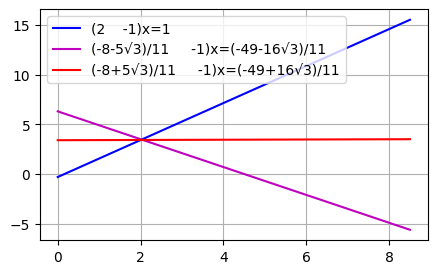
\includegraphics[width=\columnwidth]{chapters/11/10/3/12/fig/asgnt1.png}
    \caption{}
    \label{fig:11.10.3.12}
\end{figure}


\label{chapters/11/10/3/12}
\item
Find the value of $p$ so that the three lines $3x+y-2=0,px+2y-3=0$ and $2x-y-3=0$ may intersect at one point.


\textbf{Solution :}
\begin{align}  
&\myvec{
    3 &1&-2 \\
     $p$&2&-3\\
     2&-1&-3
}\\
\xrightarrow[R_3'=3R_3-2R_1]{R_2'=3R_2-pR_1}&\myvec{
    3&1&-2\\
     $0$&6-p&-9+2p\\
     0&-5&-5}\\
 \xrightarrow{R_3''=R_3(6-p)+5R_2}&\myvec{
    3&1&-2\\
     0&6-p&-9+2p\\
     0&0&-75+15p}\\
  \implies -75+15p&=0\\
    p&=5
\end{align}

\begin{figure}[H]
    \centering
    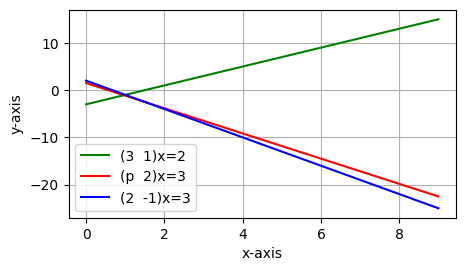
\includegraphics[width=\columnwidth]{chapters/11/10/4/9/fig/11.10.4.9.png}
    \caption{}
    \label{11.10.4.9}
\end{figure}


\label{11.10.4.9}
\item
	Show that the line through the points \brak{4,7,8},\brak{2,3,4} is parallel to the line through the points\brak{-1,-2,1},\brak{1,2,5}.

\textbf{Solution :}
For line passing through \brak{4,7,8},\brak{2,3,4},the direction vector,\begin{align}
    \vec{m_1}&=\myvec{-2\\-4\\-4}
\end{align}
For line passing through \brak{-1,-2,1},\brak{1,2,5},the direction vector,\begin{align}
    \vec{m_2}&=\myvec{2\\4\\4}
\end{align}
Therefore,the lines are parallel to each other.

	\label{12.11.2.3}
\end{enumerate}
